\documentclass[12pt]{article} %font size 12pt
\usepackage[a4paper, margin=1in]{geometry} %a4 size margin=1 inch
\usepackage{graphicx} % Required for inserting images
\usepackage{changepage}
\linespread{1} %single line spacing
\bibliographystyle{plain}
\usepackage{rotating}
\usepackage{tikz}
\usepackage{float}
\usepackage{titlesec}
\usepackage{hyperref}
\usepackage[acronym]{glossaries}
\usepackage{multirow}
\usepackage{gensymb}
\DeclareUnicodeCharacter{2060}{\nolinebreak}
\usetikzlibrary{mindmap, shapes, arrows.meta, positioning}
\usepackage{pgfgantt}
\usepackage{appendix}
\usepackage{svg}
\usepackage{tabularx}
\usepackage{dblfloatfix}
\usepackage[utf8]{inputenc}
\usepackage{graphicx}
\graphicspath{ {figures/} }
\usepackage{array}
\usepackage{color}   %May be necessary if you want to color links
\usepackage{setspace}
\usepackage{listings}
 %%%%%%%%%%%%%%%%%%%%%%%%%%%%%%%%%%%%%%%%%%%%%%%%%%%%%%%%%%%%%%%%%%%%%%%%%%%%%%%% 
%%% ~ Arduino Language - Arduino IDE Colors ~                                  %%%
%%%                                                                            %%%
%%% Kyle Rocha-Brownell | 10/2/2017 | No Licence                               %%%
%%% -------------------------------------------------------------------------- %%%
%%%                                                                            %%%
%%% Place this file in your working directory (next to the latex file you're   %%%
%%% working on).  To add it to your project, place:                            %%%
%%%     %%%%%%%%%%%%%%%%%%%%%%%%%%%%%%%%%%%%%%%%%%%%%%%%%%%%%%%%%%%%%%%%%%%%%%%%%%%%%%%% 
%%% ~ Arduino Language - Arduino IDE Colors ~                                  %%%
%%%                                                                            %%%
%%% Kyle Rocha-Brownell | 10/2/2017 | No Licence                               %%%
%%% -------------------------------------------------------------------------- %%%
%%%                                                                            %%%
%%% Place this file in your working directory (next to the latex file you're   %%%
%%% working on).  To add it to your project, place:                            %%%
%%%     %%%%%%%%%%%%%%%%%%%%%%%%%%%%%%%%%%%%%%%%%%%%%%%%%%%%%%%%%%%%%%%%%%%%%%%%%%%%%%%% 
%%% ~ Arduino Language - Arduino IDE Colors ~                                  %%%
%%%                                                                            %%%
%%% Kyle Rocha-Brownell | 10/2/2017 | No Licence                               %%%
%%% -------------------------------------------------------------------------- %%%
%%%                                                                            %%%
%%% Place this file in your working directory (next to the latex file you're   %%%
%%% working on).  To add it to your project, place:                            %%%
%%%    \input{arduinoLanguage.tex}                                             %%%
%%% somewhere before \begin{document} in your latex file.                      %%%
%%%                                                                            %%%
%%% In your document, place your arduino code between:                         %%%
%%%   \begin{lstlisting}[language=Arduino]                                     %%%
%%% and:                                                                       %%%
%%%   \end{lstlisting}                                                         %%%
%%%                                                                            %%%
%%% Or create your own style to add non-built-in functions and variables.      %%%
%%%                                                                            %%%
 %%%%%%%%%%%%%%%%%%%%%%%%%%%%%%%%%%%%%%%%%%%%%%%%%%%%%%%%%%%%%%%%%%%%%%%%%%%%%%%% 

\usepackage{color}
\usepackage{listings}    
\usepackage{courier}

%%% Define Custom IDE Colors %%%
\definecolor{arduinoGreen}    {rgb} {0.17, 0.43, 0.01}
\definecolor{arduinoGrey}     {rgb} {0.47, 0.47, 0.33}
\definecolor{arduinoOrange}   {rgb} {0.8 , 0.4 , 0   }
\definecolor{arduinoBlue}     {rgb} {0.01, 0.61, 0.98}
\definecolor{arduinoDarkBlue} {rgb} {0.0 , 0.2 , 0.5 }

%%% Define Arduino Language %%%
\lstdefinelanguage{Arduino}{
  language=C++, % begin with default C++ settings 
%
%
  %%% Keyword Color Group 1 %%%  (called KEYWORD3 by arduino)
  keywordstyle=\color{arduinoGreen},   
  deletekeywords={  % remove all arduino keywords that might be in c++
                break, case, override, final, continue, default, do, else, for, 
                if, return, goto, switch, throw, try, while, setup, loop, export, 
                not, or, and, xor, include, define, elif, else, error, if, ifdef, 
                ifndef, pragma, warning,
                HIGH, LOW, INPUT, INPUT_PULLUP, OUTPUT, DEC, BIN, HEX, OCT, PI, 
                HALF_PI, TWO_PI, LSBFIRST, MSBFIRST, CHANGE, FALLING, RISING, 
                DEFAULT, EXTERNAL, INTERNAL, INTERNAL1V1, INTERNAL2V56, LED_BUILTIN, 
                LED_BUILTIN_RX, LED_BUILTIN_TX, DIGITAL_MESSAGE, FIRMATA_STRING, 
                ANALOG_MESSAGE, REPORT_DIGITAL, REPORT_ANALOG, SET_PIN_MODE, 
                SYSTEM_RESET, SYSEX_START, auto, int8_t, int16_t, int32_t, int64_t, 
                uint8_t, uint16_t, uint32_t, uint64_t, char16_t, char32_t, operator, 
                enum, delete, bool, boolean, byte, char, const, false, float, double, 
                null, NULL, int, long, new, private, protected, public, short, 
                signed, static, volatile, String, void, true, unsigned, word, array, 
                sizeof, dynamic_cast, typedef, const_cast, struct, static_cast, union, 
                friend, extern, class, reinterpret_cast, register, explicit, inline, 
                _Bool, complex, _Complex, _Imaginary, atomic_bool, atomic_char, 
                atomic_schar, atomic_uchar, atomic_short, atomic_ushort, atomic_int, 
                atomic_uint, atomic_long, atomic_ulong, atomic_llong, atomic_ullong, 
                virtual, PROGMEM,
                Serial, Serial1, Serial2, Serial3, SerialUSB, Keyboard, Mouse,
                abs, acos, asin, atan, atan2, ceil, constrain, cos, degrees, exp, 
                floor, log, map, max, min, radians, random, randomSeed, round, sin, 
                sq, sqrt, tan, pow, bitRead, bitWrite, bitSet, bitClear, bit, 
                highByte, lowByte, analogReference, analogRead, 
                analogReadResolution, analogWrite, analogWriteResolution, 
                attachInterrupt, detachInterrupt, digitalPinToInterrupt, delay, 
                delayMicroseconds, digitalWrite, digitalRead, interrupts, millis, 
                micros, noInterrupts, noTone, pinMode, pulseIn, pulseInLong, shiftIn, 
                shiftOut, tone, yield, Stream, begin, end, peek, read, print, 
                println, available, availableForWrite, flush, setTimeout, find, 
                findUntil, parseInt, parseFloat, readBytes, readBytesUntil, readString, 
                readStringUntil, trim, toUpperCase, toLowerCase, charAt, compareTo, 
                concat, endsWith, startsWith, equals, equalsIgnoreCase, getBytes, 
                indexOf, lastIndexOf, length, replace, setCharAt, substring, 
                toCharArray, toInt, press, release, releaseAll, accept, click, move, 
                isPressed, isAlphaNumeric, isAlpha, isAscii, isWhitespace, isControl, 
                isDigit, isGraph, isLowerCase, isPrintable, isPunct, isSpace, 
                isUpperCase, isHexadecimalDigit, 
                }, 
  morekeywords={   % add arduino structures to group 1
                break, case, override, final, continue, default, do, else, for, 
                if, return, goto, switch, throw, try, while, setup, loop, export, 
                not, or, and, xor, include, define, elif, else, error, if, ifdef, 
                ifndef, pragma, warning,
                }, 
% 
%
  %%% Keyword Color Group 2 %%%  (called LITERAL1 by arduino)
  keywordstyle=[2]\color{arduinoBlue},   
  keywords=[2]{   % add variables and dataTypes as 2nd group  
                HIGH, LOW, INPUT, INPUT_PULLUP, OUTPUT, DEC, BIN, HEX, OCT, PI, 
                HALF_PI, TWO_PI, LSBFIRST, MSBFIRST, CHANGE, FALLING, RISING, 
                DEFAULT, EXTERNAL, INTERNAL, INTERNAL1V1, INTERNAL2V56, LED_BUILTIN, 
                LED_BUILTIN_RX, LED_BUILTIN_TX, DIGITAL_MESSAGE, FIRMATA_STRING, 
                ANALOG_MESSAGE, REPORT_DIGITAL, REPORT_ANALOG, SET_PIN_MODE, 
                SYSTEM_RESET, SYSEX_START, auto, int8_t, int16_t, int32_t, int64_t, 
                uint8_t, uint16_t, uint32_t, uint64_t, char16_t, char32_t, operator, 
                enum, delete, bool, boolean, byte, char, const, false, float, double, 
                null, NULL, int, long, new, private, protected, public, short, 
                signed, static, volatile, String, void, true, unsigned, word, array, 
                sizeof, dynamic_cast, typedef, const_cast, struct, static_cast, union, 
                friend, extern, class, reinterpret_cast, register, explicit, inline, 
                _Bool, complex, _Complex, _Imaginary, atomic_bool, atomic_char, 
                atomic_schar, atomic_uchar, atomic_short, atomic_ushort, atomic_int, 
                atomic_uint, atomic_long, atomic_ulong, atomic_llong, atomic_ullong, 
                virtual, PROGMEM,
                },  
% 
%
  %%% Keyword Color Group 3 %%%  (called KEYWORD1 by arduino)
  keywordstyle=[3]\bfseries\color{arduinoOrange},
  keywords=[3]{  % add built-in functions as a 3rd group
                Serial, Serial1, Serial2, Serial3, SerialUSB, Keyboard, Mouse,
                },      
%
%
  %%% Keyword Color Group 4 %%%  (called KEYWORD2 by arduino)
  keywordstyle=[4]\color{arduinoOrange},
  keywords=[4]{  % add more built-in functions as a 4th group
                abs, acos, asin, atan, atan2, ceil, constrain, cos, degrees, exp, 
                floor, log, map, max, min, radians, random, randomSeed, round, sin, 
                sq, sqrt, tan, pow, bitRead, bitWrite, bitSet, bitClear, bit, 
                highByte, lowByte, analogReference, analogRead, 
                analogReadResolution, analogWrite, analogWriteResolution, 
                attachInterrupt, detachInterrupt, digitalPinToInterrupt, delay, 
                delayMicroseconds, digitalWrite, digitalRead, interrupts, millis, 
                micros, noInterrupts, noTone, pinMode, pulseIn, pulseInLong, shiftIn, 
                shiftOut, tone, yield, Stream, begin, end, peek, read, print, 
                println, available, availableForWrite, flush, setTimeout, find, 
                findUntil, parseInt, parseFloat, readBytes, readBytesUntil, readString, 
                readStringUntil, trim, toUpperCase, toLowerCase, charAt, compareTo, 
                concat, endsWith, startsWith, equals, equalsIgnoreCase, getBytes, 
                indexOf, lastIndexOf, length, replace, setCharAt, substring, 
                toCharArray, toInt, press, release, releaseAll, accept, click, move, 
                isPressed, isAlphaNumeric, isAlpha, isAscii, isWhitespace, isControl, 
                isDigit, isGraph, isLowerCase, isPrintable, isPunct, isSpace, 
                isUpperCase, isHexadecimalDigit, 
                },      
%
%
  %%% Set Other Colors %%%
  stringstyle=\color{arduinoDarkBlue},    
  commentstyle=\color{arduinoGrey},    
%          
%   
  %%%% Line Numbering %%%%
  numbers=left,                    
  numbersep=5pt,                   
  numberstyle=\color{arduinoGrey},    
  %stepnumber=2,                      % show every 2 line numbers
%
%
  %%%% Code Box Style %%%%
  breaklines=true,                    % wordwrapping
  tabsize=2,         
  basicstyle=\ttfamily  
}
                                             %%%
%%% somewhere before \begin{document} in your latex file.                      %%%
%%%                                                                            %%%
%%% In your document, place your arduino code between:                         %%%
%%%   \begin{lstlisting}[language=Arduino]                                     %%%
%%% and:                                                                       %%%
%%%   \end{lstlisting}                                                         %%%
%%%                                                                            %%%
%%% Or create your own style to add non-built-in functions and variables.      %%%
%%%                                                                            %%%
 %%%%%%%%%%%%%%%%%%%%%%%%%%%%%%%%%%%%%%%%%%%%%%%%%%%%%%%%%%%%%%%%%%%%%%%%%%%%%%%% 

\usepackage{color}
\usepackage{listings}    
\usepackage{courier}

%%% Define Custom IDE Colors %%%
\definecolor{arduinoGreen}    {rgb} {0.17, 0.43, 0.01}
\definecolor{arduinoGrey}     {rgb} {0.47, 0.47, 0.33}
\definecolor{arduinoOrange}   {rgb} {0.8 , 0.4 , 0   }
\definecolor{arduinoBlue}     {rgb} {0.01, 0.61, 0.98}
\definecolor{arduinoDarkBlue} {rgb} {0.0 , 0.2 , 0.5 }

%%% Define Arduino Language %%%
\lstdefinelanguage{Arduino}{
  language=C++, % begin with default C++ settings 
%
%
  %%% Keyword Color Group 1 %%%  (called KEYWORD3 by arduino)
  keywordstyle=\color{arduinoGreen},   
  deletekeywords={  % remove all arduino keywords that might be in c++
                break, case, override, final, continue, default, do, else, for, 
                if, return, goto, switch, throw, try, while, setup, loop, export, 
                not, or, and, xor, include, define, elif, else, error, if, ifdef, 
                ifndef, pragma, warning,
                HIGH, LOW, INPUT, INPUT_PULLUP, OUTPUT, DEC, BIN, HEX, OCT, PI, 
                HALF_PI, TWO_PI, LSBFIRST, MSBFIRST, CHANGE, FALLING, RISING, 
                DEFAULT, EXTERNAL, INTERNAL, INTERNAL1V1, INTERNAL2V56, LED_BUILTIN, 
                LED_BUILTIN_RX, LED_BUILTIN_TX, DIGITAL_MESSAGE, FIRMATA_STRING, 
                ANALOG_MESSAGE, REPORT_DIGITAL, REPORT_ANALOG, SET_PIN_MODE, 
                SYSTEM_RESET, SYSEX_START, auto, int8_t, int16_t, int32_t, int64_t, 
                uint8_t, uint16_t, uint32_t, uint64_t, char16_t, char32_t, operator, 
                enum, delete, bool, boolean, byte, char, const, false, float, double, 
                null, NULL, int, long, new, private, protected, public, short, 
                signed, static, volatile, String, void, true, unsigned, word, array, 
                sizeof, dynamic_cast, typedef, const_cast, struct, static_cast, union, 
                friend, extern, class, reinterpret_cast, register, explicit, inline, 
                _Bool, complex, _Complex, _Imaginary, atomic_bool, atomic_char, 
                atomic_schar, atomic_uchar, atomic_short, atomic_ushort, atomic_int, 
                atomic_uint, atomic_long, atomic_ulong, atomic_llong, atomic_ullong, 
                virtual, PROGMEM,
                Serial, Serial1, Serial2, Serial3, SerialUSB, Keyboard, Mouse,
                abs, acos, asin, atan, atan2, ceil, constrain, cos, degrees, exp, 
                floor, log, map, max, min, radians, random, randomSeed, round, sin, 
                sq, sqrt, tan, pow, bitRead, bitWrite, bitSet, bitClear, bit, 
                highByte, lowByte, analogReference, analogRead, 
                analogReadResolution, analogWrite, analogWriteResolution, 
                attachInterrupt, detachInterrupt, digitalPinToInterrupt, delay, 
                delayMicroseconds, digitalWrite, digitalRead, interrupts, millis, 
                micros, noInterrupts, noTone, pinMode, pulseIn, pulseInLong, shiftIn, 
                shiftOut, tone, yield, Stream, begin, end, peek, read, print, 
                println, available, availableForWrite, flush, setTimeout, find, 
                findUntil, parseInt, parseFloat, readBytes, readBytesUntil, readString, 
                readStringUntil, trim, toUpperCase, toLowerCase, charAt, compareTo, 
                concat, endsWith, startsWith, equals, equalsIgnoreCase, getBytes, 
                indexOf, lastIndexOf, length, replace, setCharAt, substring, 
                toCharArray, toInt, press, release, releaseAll, accept, click, move, 
                isPressed, isAlphaNumeric, isAlpha, isAscii, isWhitespace, isControl, 
                isDigit, isGraph, isLowerCase, isPrintable, isPunct, isSpace, 
                isUpperCase, isHexadecimalDigit, 
                }, 
  morekeywords={   % add arduino structures to group 1
                break, case, override, final, continue, default, do, else, for, 
                if, return, goto, switch, throw, try, while, setup, loop, export, 
                not, or, and, xor, include, define, elif, else, error, if, ifdef, 
                ifndef, pragma, warning,
                }, 
% 
%
  %%% Keyword Color Group 2 %%%  (called LITERAL1 by arduino)
  keywordstyle=[2]\color{arduinoBlue},   
  keywords=[2]{   % add variables and dataTypes as 2nd group  
                HIGH, LOW, INPUT, INPUT_PULLUP, OUTPUT, DEC, BIN, HEX, OCT, PI, 
                HALF_PI, TWO_PI, LSBFIRST, MSBFIRST, CHANGE, FALLING, RISING, 
                DEFAULT, EXTERNAL, INTERNAL, INTERNAL1V1, INTERNAL2V56, LED_BUILTIN, 
                LED_BUILTIN_RX, LED_BUILTIN_TX, DIGITAL_MESSAGE, FIRMATA_STRING, 
                ANALOG_MESSAGE, REPORT_DIGITAL, REPORT_ANALOG, SET_PIN_MODE, 
                SYSTEM_RESET, SYSEX_START, auto, int8_t, int16_t, int32_t, int64_t, 
                uint8_t, uint16_t, uint32_t, uint64_t, char16_t, char32_t, operator, 
                enum, delete, bool, boolean, byte, char, const, false, float, double, 
                null, NULL, int, long, new, private, protected, public, short, 
                signed, static, volatile, String, void, true, unsigned, word, array, 
                sizeof, dynamic_cast, typedef, const_cast, struct, static_cast, union, 
                friend, extern, class, reinterpret_cast, register, explicit, inline, 
                _Bool, complex, _Complex, _Imaginary, atomic_bool, atomic_char, 
                atomic_schar, atomic_uchar, atomic_short, atomic_ushort, atomic_int, 
                atomic_uint, atomic_long, atomic_ulong, atomic_llong, atomic_ullong, 
                virtual, PROGMEM,
                },  
% 
%
  %%% Keyword Color Group 3 %%%  (called KEYWORD1 by arduino)
  keywordstyle=[3]\bfseries\color{arduinoOrange},
  keywords=[3]{  % add built-in functions as a 3rd group
                Serial, Serial1, Serial2, Serial3, SerialUSB, Keyboard, Mouse,
                },      
%
%
  %%% Keyword Color Group 4 %%%  (called KEYWORD2 by arduino)
  keywordstyle=[4]\color{arduinoOrange},
  keywords=[4]{  % add more built-in functions as a 4th group
                abs, acos, asin, atan, atan2, ceil, constrain, cos, degrees, exp, 
                floor, log, map, max, min, radians, random, randomSeed, round, sin, 
                sq, sqrt, tan, pow, bitRead, bitWrite, bitSet, bitClear, bit, 
                highByte, lowByte, analogReference, analogRead, 
                analogReadResolution, analogWrite, analogWriteResolution, 
                attachInterrupt, detachInterrupt, digitalPinToInterrupt, delay, 
                delayMicroseconds, digitalWrite, digitalRead, interrupts, millis, 
                micros, noInterrupts, noTone, pinMode, pulseIn, pulseInLong, shiftIn, 
                shiftOut, tone, yield, Stream, begin, end, peek, read, print, 
                println, available, availableForWrite, flush, setTimeout, find, 
                findUntil, parseInt, parseFloat, readBytes, readBytesUntil, readString, 
                readStringUntil, trim, toUpperCase, toLowerCase, charAt, compareTo, 
                concat, endsWith, startsWith, equals, equalsIgnoreCase, getBytes, 
                indexOf, lastIndexOf, length, replace, setCharAt, substring, 
                toCharArray, toInt, press, release, releaseAll, accept, click, move, 
                isPressed, isAlphaNumeric, isAlpha, isAscii, isWhitespace, isControl, 
                isDigit, isGraph, isLowerCase, isPrintable, isPunct, isSpace, 
                isUpperCase, isHexadecimalDigit, 
                },      
%
%
  %%% Set Other Colors %%%
  stringstyle=\color{arduinoDarkBlue},    
  commentstyle=\color{arduinoGrey},    
%          
%   
  %%%% Line Numbering %%%%
  numbers=left,                    
  numbersep=5pt,                   
  numberstyle=\color{arduinoGrey},    
  %stepnumber=2,                      % show every 2 line numbers
%
%
  %%%% Code Box Style %%%%
  breaklines=true,                    % wordwrapping
  tabsize=2,         
  basicstyle=\ttfamily  
}
                                             %%%
%%% somewhere before \begin{document} in your latex file.                      %%%
%%%                                                                            %%%
%%% In your document, place your arduino code between:                         %%%
%%%   \begin{lstlisting}[language=Arduino]                                     %%%
%%% and:                                                                       %%%
%%%   \end{lstlisting}                                                         %%%
%%%                                                                            %%%
%%% Or create your own style to add non-built-in functions and variables.      %%%
%%%                                                                            %%%
 %%%%%%%%%%%%%%%%%%%%%%%%%%%%%%%%%%%%%%%%%%%%%%%%%%%%%%%%%%%%%%%%%%%%%%%%%%%%%%%% 

\usepackage{color}
\usepackage{listings}    
\usepackage{courier}

%%% Define Custom IDE Colors %%%
\definecolor{arduinoGreen}    {rgb} {0.17, 0.43, 0.01}
\definecolor{arduinoGrey}     {rgb} {0.47, 0.47, 0.33}
\definecolor{arduinoOrange}   {rgb} {0.8 , 0.4 , 0   }
\definecolor{arduinoBlue}     {rgb} {0.01, 0.61, 0.98}
\definecolor{arduinoDarkBlue} {rgb} {0.0 , 0.2 , 0.5 }

%%% Define Arduino Language %%%
\lstdefinelanguage{Arduino}{
  language=C++, % begin with default C++ settings 
%
%
  %%% Keyword Color Group 1 %%%  (called KEYWORD3 by arduino)
  keywordstyle=\color{arduinoGreen},   
  deletekeywords={  % remove all arduino keywords that might be in c++
                break, case, override, final, continue, default, do, else, for, 
                if, return, goto, switch, throw, try, while, setup, loop, export, 
                not, or, and, xor, include, define, elif, else, error, if, ifdef, 
                ifndef, pragma, warning,
                HIGH, LOW, INPUT, INPUT_PULLUP, OUTPUT, DEC, BIN, HEX, OCT, PI, 
                HALF_PI, TWO_PI, LSBFIRST, MSBFIRST, CHANGE, FALLING, RISING, 
                DEFAULT, EXTERNAL, INTERNAL, INTERNAL1V1, INTERNAL2V56, LED_BUILTIN, 
                LED_BUILTIN_RX, LED_BUILTIN_TX, DIGITAL_MESSAGE, FIRMATA_STRING, 
                ANALOG_MESSAGE, REPORT_DIGITAL, REPORT_ANALOG, SET_PIN_MODE, 
                SYSTEM_RESET, SYSEX_START, auto, int8_t, int16_t, int32_t, int64_t, 
                uint8_t, uint16_t, uint32_t, uint64_t, char16_t, char32_t, operator, 
                enum, delete, bool, boolean, byte, char, const, false, float, double, 
                null, NULL, int, long, new, private, protected, public, short, 
                signed, static, volatile, String, void, true, unsigned, word, array, 
                sizeof, dynamic_cast, typedef, const_cast, struct, static_cast, union, 
                friend, extern, class, reinterpret_cast, register, explicit, inline, 
                _Bool, complex, _Complex, _Imaginary, atomic_bool, atomic_char, 
                atomic_schar, atomic_uchar, atomic_short, atomic_ushort, atomic_int, 
                atomic_uint, atomic_long, atomic_ulong, atomic_llong, atomic_ullong, 
                virtual, PROGMEM,
                Serial, Serial1, Serial2, Serial3, SerialUSB, Keyboard, Mouse,
                abs, acos, asin, atan, atan2, ceil, constrain, cos, degrees, exp, 
                floor, log, map, max, min, radians, random, randomSeed, round, sin, 
                sq, sqrt, tan, pow, bitRead, bitWrite, bitSet, bitClear, bit, 
                highByte, lowByte, analogReference, analogRead, 
                analogReadResolution, analogWrite, analogWriteResolution, 
                attachInterrupt, detachInterrupt, digitalPinToInterrupt, delay, 
                delayMicroseconds, digitalWrite, digitalRead, interrupts, millis, 
                micros, noInterrupts, noTone, pinMode, pulseIn, pulseInLong, shiftIn, 
                shiftOut, tone, yield, Stream, begin, end, peek, read, print, 
                println, available, availableForWrite, flush, setTimeout, find, 
                findUntil, parseInt, parseFloat, readBytes, readBytesUntil, readString, 
                readStringUntil, trim, toUpperCase, toLowerCase, charAt, compareTo, 
                concat, endsWith, startsWith, equals, equalsIgnoreCase, getBytes, 
                indexOf, lastIndexOf, length, replace, setCharAt, substring, 
                toCharArray, toInt, press, release, releaseAll, accept, click, move, 
                isPressed, isAlphaNumeric, isAlpha, isAscii, isWhitespace, isControl, 
                isDigit, isGraph, isLowerCase, isPrintable, isPunct, isSpace, 
                isUpperCase, isHexadecimalDigit, 
                }, 
  morekeywords={   % add arduino structures to group 1
                break, case, override, final, continue, default, do, else, for, 
                if, return, goto, switch, throw, try, while, setup, loop, export, 
                not, or, and, xor, include, define, elif, else, error, if, ifdef, 
                ifndef, pragma, warning,
                }, 
% 
%
  %%% Keyword Color Group 2 %%%  (called LITERAL1 by arduino)
  keywordstyle=[2]\color{arduinoBlue},   
  keywords=[2]{   % add variables and dataTypes as 2nd group  
                HIGH, LOW, INPUT, INPUT_PULLUP, OUTPUT, DEC, BIN, HEX, OCT, PI, 
                HALF_PI, TWO_PI, LSBFIRST, MSBFIRST, CHANGE, FALLING, RISING, 
                DEFAULT, EXTERNAL, INTERNAL, INTERNAL1V1, INTERNAL2V56, LED_BUILTIN, 
                LED_BUILTIN_RX, LED_BUILTIN_TX, DIGITAL_MESSAGE, FIRMATA_STRING, 
                ANALOG_MESSAGE, REPORT_DIGITAL, REPORT_ANALOG, SET_PIN_MODE, 
                SYSTEM_RESET, SYSEX_START, auto, int8_t, int16_t, int32_t, int64_t, 
                uint8_t, uint16_t, uint32_t, uint64_t, char16_t, char32_t, operator, 
                enum, delete, bool, boolean, byte, char, const, false, float, double, 
                null, NULL, int, long, new, private, protected, public, short, 
                signed, static, volatile, String, void, true, unsigned, word, array, 
                sizeof, dynamic_cast, typedef, const_cast, struct, static_cast, union, 
                friend, extern, class, reinterpret_cast, register, explicit, inline, 
                _Bool, complex, _Complex, _Imaginary, atomic_bool, atomic_char, 
                atomic_schar, atomic_uchar, atomic_short, atomic_ushort, atomic_int, 
                atomic_uint, atomic_long, atomic_ulong, atomic_llong, atomic_ullong, 
                virtual, PROGMEM,
                },  
% 
%
  %%% Keyword Color Group 3 %%%  (called KEYWORD1 by arduino)
  keywordstyle=[3]\bfseries\color{arduinoOrange},
  keywords=[3]{  % add built-in functions as a 3rd group
                Serial, Serial1, Serial2, Serial3, SerialUSB, Keyboard, Mouse,
                },      
%
%
  %%% Keyword Color Group 4 %%%  (called KEYWORD2 by arduino)
  keywordstyle=[4]\color{arduinoOrange},
  keywords=[4]{  % add more built-in functions as a 4th group
                abs, acos, asin, atan, atan2, ceil, constrain, cos, degrees, exp, 
                floor, log, map, max, min, radians, random, randomSeed, round, sin, 
                sq, sqrt, tan, pow, bitRead, bitWrite, bitSet, bitClear, bit, 
                highByte, lowByte, analogReference, analogRead, 
                analogReadResolution, analogWrite, analogWriteResolution, 
                attachInterrupt, detachInterrupt, digitalPinToInterrupt, delay, 
                delayMicroseconds, digitalWrite, digitalRead, interrupts, millis, 
                micros, noInterrupts, noTone, pinMode, pulseIn, pulseInLong, shiftIn, 
                shiftOut, tone, yield, Stream, begin, end, peek, read, print, 
                println, available, availableForWrite, flush, setTimeout, find, 
                findUntil, parseInt, parseFloat, readBytes, readBytesUntil, readString, 
                readStringUntil, trim, toUpperCase, toLowerCase, charAt, compareTo, 
                concat, endsWith, startsWith, equals, equalsIgnoreCase, getBytes, 
                indexOf, lastIndexOf, length, replace, setCharAt, substring, 
                toCharArray, toInt, press, release, releaseAll, accept, click, move, 
                isPressed, isAlphaNumeric, isAlpha, isAscii, isWhitespace, isControl, 
                isDigit, isGraph, isLowerCase, isPrintable, isPunct, isSpace, 
                isUpperCase, isHexadecimalDigit, 
                },      
%
%
  %%% Set Other Colors %%%
  stringstyle=\color{arduinoDarkBlue},    
  commentstyle=\color{arduinoGrey},    
%          
%   
  %%%% Line Numbering %%%%
  numbers=left,                    
  numbersep=5pt,                   
  numberstyle=\color{arduinoGrey},    
  %stepnumber=2,                      % show every 2 line numbers
%
%
  %%%% Code Box Style %%%%
  breaklines=true,                    % wordwrapping
  tabsize=2,         
  basicstyle=\ttfamily  
}
    % adds the arduino language listing
\usepackage{xcolor}

\definecolor{codegreen}{rgb}{0,0.6,0}
\definecolor{codegray}{rgb}{0.5,0.5,0.5}
\definecolor{codepurple}{rgb}{0.58,0,0.82}
\definecolor{backcolour}{rgb}{0.95,0.95,0.92}

\lstdefinestyle{myArduino}{
    language=Arduino,
    backgroundcolor=\color{backcolour},   
    commentstyle=\color{codegreen},
    keywordstyle=\color{magenta},
    numberstyle=\tiny\color{codegray},
    stringstyle=\color{codepurple},
    basicstyle=\ttfamily\footnotesize,
    breakatwhitespace=false,         
    breaklines=true,                 
    captionpos=b,                    
    keepspaces=true,                 
    numbers=left,                    
    numbersep=5pt,                  
    showspaces=false,                
    showstringspaces=false,
    showtabs=false,                  
    tabsize=2
}

\lstset{style=myArduino}



\usepackage[load-configurations = abbreviations]{siunitx}
\usepackage[acronym]{glossaries}
\usepackage{imakeidx}
\usepackage{tabularx}
\makeindex[columns=3, title=Index,intoc]
\hypersetup{
    colorlinks=true, %set true if you want colored links
    linktoc=all,     %set to all if you want both sections and subsections linked
    linkcolor=blue,  % Choose some color if you want links to stand out
}

\makeglossaries
\newglossaryentry{Accelerometer}
{
        name=Accelerometer,
        description={An accelerometer is a device that measures the vibration, or acceleration of motion, of a structure}
}
\newglossaryentry{IP67}
{
        name=IP67,
        description={An IP67 rated enclosure offers dust tight protection against solid ingress from sources like windblown dirt. Combine that with strong water resistance to everything from hose sprays to temporary submersion, and it's easy to see why designers often specify IP67 enclosures for their devices.}
}
\newglossaryentry{ESP32}
{
        name=ESP32,
        description={ESP32 is a series of low-cost, low-power system on a chip microcontrollers with integrated Wi-Fi and dual-mode Bluetooth.}
}
\newglossaryentry{MPU 6050}
{
        name=MPU 6050,
        description={The MPU-6050 devices combine a 3-axis gyroscope and a 3-axis accelerometer on the same silicon die, together with an onboard Digital Motion Processor™ (DMP™), which processes complex 6-axis MotionFusion algorithms.}
}
\newglossaryentry{gyrometer}
{
        name=Gyrometer,
        description={Gyrometers compliment accelerometers as game controllers. The accelerometer can measure linear motion while the gyrometer measures angular velocity or rotational motion. Note. For a more complete implementation, see the gyrometer sample.}
}

\newacronym{if}{IF}{Involvement Factor}
\newacronym{ac}{AC}{Activity Coordinator}
\newacronym{tc}{TC}{Tribe Coordinator}
\newacronym{WBS}{WBS}{Work Breakdown Structure}
\newacronym{TRL}{TRL}{Technology Readiness Level}
\newacronym{inr}{INR}{Indian National Rupees}
\newacronym{bu}{BU}{Bus Unit}
\newacronym{lcd}{LCD}{Liquid Crystal Display}
\newacronym{led}{LED}{Light Emitting Diode}
\newacronym{gsm}{GSM}{Global System for Mobile Communication}
\newacronym{ble}{BLE}{Bluetooth Low Energy}
\newacronym{pir}{PIR}{Passive Infrared Sensor}
\newacronym{cad}{CAD}{Computer Aided Design}
\newacronym{buk}{BUk}{k'th Bus Unit}
\newacronym{PWM}{PWM}{Pulse-Width Modulation}

\setcounter{secnumdepth}{4}

\titleformat{\paragraph}
{\normalfont\normalsize\bfseries}{\theparagraph}{1em}{}
\titlespacing*{\paragraph}
{0pt}{3.25ex plus 1ex minus .2ex}{1.5ex plus .2ex}
%\usepackage[style=apa, backend=biber]{biblatex}
%\addbibresource{ref.bib}

\begin{document}
\begin{titlepage}
\thispagestyle{empty}
\centering

\includegraphics[width=0.3\textwidth]{logo.png}
\\
\large{Indian Institute of Technology Delhi, New Delhi}
\vfill
\centering
\vspace{7pt}
\setstretch{2}
{\huge\textbf{ELP305-Submission-2:\\ Project 2: SmartBus\\}}
{\Large\ Enhancing Intra-Campus Transportation at IIT Delhi}
{\LARGE{\textbf{Requirements . Specifications . Design} \\ v0.2}}
\\

{\large{TRIBE B}}


\vspace{0.5cm}
\Huge\textbf{}
\vspace{0.1cm}
\vfill
%\large{Contact: \\}
\large{27 April, 2024\\}
\large{Document ID: 2024-04-02-335691\\}



\end{titlepage}



\clearpage
\section{Tribe B Team Member Details}
\subsection{Tribe B Members with  \acrshort{if} = 1}
\begin{table}[h!]
\centering

\begin{tabular}{|c|r|r|c|r|}
\hline
Name & Entry No & Email & Role & \acrshort{if} \\
\hline
Subham & 2022MT11823 & \href{mailto:mt1221823@maths.iitd.ac.in}{mt1221823@maths.iitd.ac.in} & \acrshort{tc} & 1 \\
Aditi Srivastava & 2021MT10228 & \href{mailto:mt1210228@maths.iitd.ac.in}{mt1210228@maths.iitd.ac.in} & \acrshort{tc} & 1 \\
\hline
\end{tabular}
\caption{Tribe Coordinator Details}
\label{tab:teamDetails}
\end{table}


\begin{table}[h!]
\centering
\begin{tabular}{|c|r|r|c|r|}
\hline
Name & Entry No & Email & Role & \acrshort{if} \\
\hline
Bhumi Gadhavi & 2021MT60950 & \href{mailto:mt6210950@maths.iitd.ac.in}{mt6210950@maths.iitd.ac.in} & \acrshort{ac} & 1 \\
Pramsu Shrivastava & 2021EE10140 & \href{mailto:ee1210140@ee.iitd.ac.in}{ee1210140@ee.iitd.ac.in} & \acrshort{ac} & 1 \\
Himanshu Ghusinga & 2021MT10936 & \href{mailto:mt1210936@maths.iitd.ac.in}{mt1210936@maths.iitd.ac.in} & \acrshort{ac} & 1\\
Abhay Yadav & 2021EE10151 & \href{mailto:ee1210151@ee.iitd.ac.in}{ee1210151@ee.iitd.ac.in} & Member & 1 \\
Vaibhav Sobti & 2021EE10641 & \href{mailto:ee1210641@ee.iitd.ac.in}{ee1210641@ee.iitd.ac.in} & Member & 1 \\

Parth Naikwad & 2021EE10672 & \href{mailto:ee1210672@ee.iitd.ac.in}{ee1210672@ee.iitd.ac.in} & Member & 1 \\
Yash Bafna & 2021EE10660 & \href{mailto:ee1210660@ee.iitd.ac.in}{ee1210660@ee.iitd.ac.in} & Member & 1 \\
S Anuj Karthik & 2021EE10667 & \href{mailto:ee1210667@ee.iitd.ac.in}{ee1210667@ee.iitd.ac.in} & Member & 1 \\

Tushar Daima & 2021EE10688 & \href{mailto:ee1210688@ee.iitd.ac.in}{ee1210688@ee.iitd.ac.in} & Member & 1 \\
Tanisha Chouhan & 2021EE10693 & \href{mailto:ee1210693@ee.iitd.ac.in}{ee1210693@ee.iitd.ac.in} & Member & 1 \\
Drishti Gupta & 2021EE10649 & \href{mailto:ee1210649@ee.iitd.ac.in}{ee1210649@ee.iitd.ac.in} & Member & 1 \\
Ridhima Gupta & 2021EE30719 & \href{mailto:ee3210719@ee.iitd.ac.in}{ee3210719@ee.iitd.ac.in} & Member & 1 \\
Diksha & 2021EE30717 & \href{mailto:ee3210717@ee.iitd.ac.in}{ee3210717@ee.iitd.ac.in} & Member & 1 \\
Sanju N S & 2021EE30732 & \href{mailto:ee3210732@ee.iitd.ac.in}{ee3210732@ee.iitd.ac.in} & Member & 1 \\
Deepak Kumar & 2021EE10152 & \href{mailto:ee1210152@ee.iitd.ac.in}{ee1210152@ee.iitd.ac.in} & Member & 1 \\
Rishika Goel & 2021EE30725 & \href{mailto:ee32107255@ee.iitd.ac.in}{ee3210725@ee.iitd.ac.in} & Member & 1 \\

Narendra Nath Sharma & 2021EE10695 & \href{mailto:ee1210695@ee.iitd.ac.in}{ee1210695@ee.iitd.ac.in} & Member & 1 \\
Tanmay Jhalani & 2021EE30389 & \href{mailto:ee3210389@ee.iitd.ac.in}{ee3210389@ee.iitd.ac.in} & Member & 1 \\
Anish Gupta & 2021EE10663 & \href{mailto:ee1210663@ee.iitd.ac.in}{ee1210663@ee.iitd.ac.in} & Member & 1 \\
Ram Chaudhari & 2021EE10671 & \href{mailto:ee1210671@ee.iitd.ac.in}{ee1210671@ee.iitd.ac.in} & Member & 1 \\

Shantanu Pandit & 2021MT10252 & \href{mailto:mt1210252@maths.iitd.ac.in}{mt1210252@maths.iitd.ac.in} & Member & 1 \\
Keshav Singhal & 2021EE10788 & \href{mailto:ee1210788@ee.iitd.ac.in}{ee1210788@ee.iitd.ac.in} & Member & 1 \\
Ridam Kumari & 2021EE10158 & \href{mailto:ee1210158@ee.iitd.ac.in}{ee1210158@ee.iitd.ac.in} & Member & 1 \\

\hline
\end{tabular}
\caption{Design Team Members Details with \acrshort{if} = 1}
\label{tab:teamDetails}
\end{table}








\begin{table}[h!]
\centering
\begin{tabular}{|c|r|r|c|r|}
\hline
Name & Entry No & Email & Role & \acrshort{if} \\
\hline
Ashi Veerman & 2021MT10241 & \href{mailto:mt1210241@maths.iitd.ac.in}{mt1210241@maths.iitd.ac.in} & \acrshort{ac} & 1 \\
Rakshitha & 2021MT10904 & \href{mailto:mt1210904@maths.iitd.ac.in}{mt1210904@maths.iitd.ac.in} & Member & 1 \\
Shreya Gupta & 2021MT10906 & \href{mailto:mt1210906@maths.iitd.ac.in}{mt1210906@maths.iitd.ac.in} & Member & 1 \\
Priyal Jain & 2021MT60949 & \href{mailto:mt6210949@maths.iitd.ac.in}{mt6210949@maths.iitd.ac.in} & Member & 1 \\
Aditya Thomas & 2021MT60944 & \href{mailto:mt6210944@maths.iitd.ac.in}{mt6210944@maths.iitd.ac.in} & Member & 1 \\
Bhargab Sonowal & 2021MT10937 & \href{mailto:mt1210937@maths.iitd.ac.in}{mt1210937@maths.iitd.ac.in} & Member & 1 \\
Sanjay Karela & 2012MT50616 & \href{mailto:mt5120616@maths.iitd.ac.in}{mt5120616@maths.iitd.ac.in} & Member & 1\\


\hline
\end{tabular}
\caption{Documentation Team Members Details with \acrshort{if} = 1}
\label{tab:teamDetails}
\end{table}



\subsection{Tribe B Members with  \acrshort{if} $<$ 1}

\begin{table}[H]
\centering
\resizebox{\columnwidth}{!}{%
\begin{tabular}{|c|r|r|c|r|c|}
\hline
Name & Entry No & Email & Role & \acrshort{if} & Justification \\
\hline
Dhruv Nagpal & 2020EE11013 & \href{mailto:ee1201013@ee.iitd.ac.in}{ee1201013@ee.iitd.ac.in} & Member & 0.5 & Hour-based formula\\
Raswanth J & 2021EE30179 & \href{mailto:ee3210179@ee.iitd.ac.in}{ee3210179@ee.iitd.ac.in} & Member & 0.8 & Hour-based formula\\
Harsh Bagde & 2021EE10690 & \href{mailto:ee1210690@ee.iitd.ac.in}{ee1210690@ee.iitd.ac.in} & Member & 0.8 & Hour-based formula\\
Manan Singal & 2021EE10138 & \href{mailto:ee1210138@ee.iitd.ac.in}{ee1210138@ee.iitd.ac.in} & Member & 0.8 & Hour-based formula\\
Varshith Reddy Ryala & 2021EE10142 & \href{mailto:ee1210142@ee.iitd.ac.in}{ee1210142@ee.iitd.ac.in} & Member & 0.8 & Hour-based formula\\
Stuti Anand & 2021EE30748 & \href{mailto:ee3210748@ee.iitd.ac.in}{ee3210748@ee.iitd.ac.in} & Member & 0.8 & Hour-based formula\\
Praveen Srivastava & 2021EE10133 & \href{mailto:ee1210133@ee.iitd.ac.in}{ee1210133@ee.iitd.ac.in} & Member & 0.8 & Hour-based formula\\
Dhruv Mittal & 2021EE10626 & \href{mailto:ee1210626@ee.iitd.ac.in}{ee1210626@ee.iitd.ac.in} & Member & 0.8 & Hour-based formula \\
Pratibha Patel & 2021EE10681 & \href{mailto:ee1210681@ee.iitd.ac.in}{ee1210681@ee.iitd.ac.in} & Member  & 0.8 & Hour-based formula \\
Siddhika Tailor & 2021EE10683 & \href{mailto:ee1210683@ee.iitd.ac.in}{ee1210683@ee.iitd.ac.in} & Member& 0.8 & Hour-based formula \\
Anmol Bansal & 2021EE10643 & \href{mailto:ee1210643@ee.iitd.ac.in}{ee1210643@ee.iitd.ac.in} & Member & 0.8 & Hour-based formula \\
Kinshuk Bansal & 2021EE30701 & \href{mailto:ee3210701@ee.iitd.ac.in}{ee3210701@ee.iitd.ac.in} & Member & 0.7 & Hour-based formula\\
Divyansh Bhatnagar & 2021EE30721 & \href{mailto:ee3210721@ee.iitd.ac.in}{ee3210721@ee.iitd.ac.in} & Member & 0.7 & Hour-based formula \\
Aaditya Pratap Singh & 2019MT60737 & \href{mailto:mt6190737@maths.iitd.ac.in}{mt6190737@maths.iitd.ac.in} & Member & 0.3 & Hour-based formula\\
Ayush Singh & 2021EE30180 & \href{mailto:ee3210180@ee.iitd.ac.in}{ee3210180@ee.iitd.ac.in} & Member & 0.3 & Hour-based formula \\
Vivek Pratap Singh & 2021EE10687 & \href{mailto:ee1210687@ee.iitd.ac.in}{ee1210687@ee.iitd.ac.in} & Member & 0.7 & Hour-based formula \\
Vedant Kokate & 2021EE10631 & \href{mailto:ee1210631@ee.iitd.ac.in}{ee1210631@ee.iitd.ac.in} & Member & 0.8 & Hour-based formula\\
Ranjeet Mishra & 2021EE10656 & \href{mailto:ee12106568@maths.iitd.ac.in}{ee12106568@ee.iitd.ac.in} & Member & 0.7 & Hour-based formula\\
Vedant Patel & 2021EE10520 & \href{mailto:ee1210520@ee.iitd.ac.in}{ee1210520@ee.iitd.ac.in} & Member & 0.8 & Hour-based formula \\
Siddharth & 2022MT62028 & \href{mailto:mt6222028@maths.iitd.ac.in}{mt6222028@maths.iitd.ac.in} & Member & 0.7 & Hour-based formula\\
Mridul Jagrat & 2021EE30182 & \href{mailto:ee3210182@ee.iitd.ac.in}{ee3210182@ee.iitd.ac.in} & Member & 0.8 & Hour-based formula\\
Nidhish & 2021EE30176 & \href{mailto:ee3210176@ee.iitd.ac.in}{ee3210176@ee.iitd.ac.in} & Member & 0.8 & Hour-based formula\\
Abhishek Meena & 2021EE10172 & \href{mailto:ee1210172@ee.iitd.ac.in}{ee1210172@ee.iitd.ac.in} & Member & 0.3 & Hour-based formula\\
\hline
\end{tabular}%
}
\caption{Design and Fabrication Team Members Details with \acrshort{if} $<$ 1}
\label{tab:teamDetails}
\end{table}


% \begin{table}[h!]
% \centering
% \resizebox{\columnwidth}{!}{%
% \begin{tabular}{|c|r|r|c|r|c|}
% \hline
% Name & Entry No & Email & Role & \acrshort{if} & Justification \\
% \hline
% Rishika Goel & 2021EE30725 & \href{mailto:ee3210725@ee.iitd.ac.in}{ee3210725@ee.iitd.ac.in} & Member & 0.79 & Hour-based formula \\
% Nidhish & 2021EE30176 & \href{mailto:ee3210176@ee.iitd.ac.in}{ee3210176@ee.iitd.ac.in} & Member & 0.65 & Hour-based formula \\
% Priyal Jain & 2021MT60949 & \href{mailto:mt6210949@maths.iitd.ac.in}{mt6210949@maths.iitd.ac.in} & Member & 0.93 & Hour-based formula \\
% Aditya Thomas & 2021MT60944 & \href{mailto:mt6210944@maths.iitd.ac.in}{mt6210944@maths.iitd.ac.in} & Member & 0.93 & Hour-based formula \\
% Narendra Nath Sharma & 2021EE10695 & \href{mailto:ee1210695@ee.iitd.ac.in}{ee1210695@ee.iitd.ac.in} & Member & 0.65 & Hour-based formula \\
% Stuti Anand & 2021EE30748 & \href{mailto:ee3210748@ee.iitd.ac.in}{ee3210748@ee.iitd.ac.in} & Member & 0.79 & Hour-based formula\\
% Anish Gupta & 2021EE10663 & \href{mailto:ee1210663@ee.iitd.ac.in}{ee1210663@ee.iitd.ac.in} & Member & 0.79 & Hour-based formula \\
% Mridul Jagrat & 2021EE30182 & \href{mailto:ee3210182@ee.iitd.ac.in}{ee3210182@ee.iitd.ac.in} & Member & 0.79 & Hour-based formula \\
% Abhishek Meena & 2021EE10172 & \href{mailto:ee1210172@ee.iitd.ac.in}{ee1210172@ee.iitd.ac.in} & Member & 0.72 & Hour-based formula \\
% Kinshuk Bansal & 2021EE30701 & \href{mailto:ee3210701@ee.iitd.ac.in}{ee3210701@ee.iitd.ac.in} & Member & 0.22 & Hour-based formula \\
% \hline
% \end{tabular}%
% }
% \caption{Research Team Members Details with \acrshort{if} $<$ 1}
% \label{tab:teamDetails}
% \end{table}

\section*{}


\clearpage
\tableofcontents

\clearpage
\listoftables
\listoffigures

\clearpage

\begin{sidewaysfigure}[htbp]
\centering
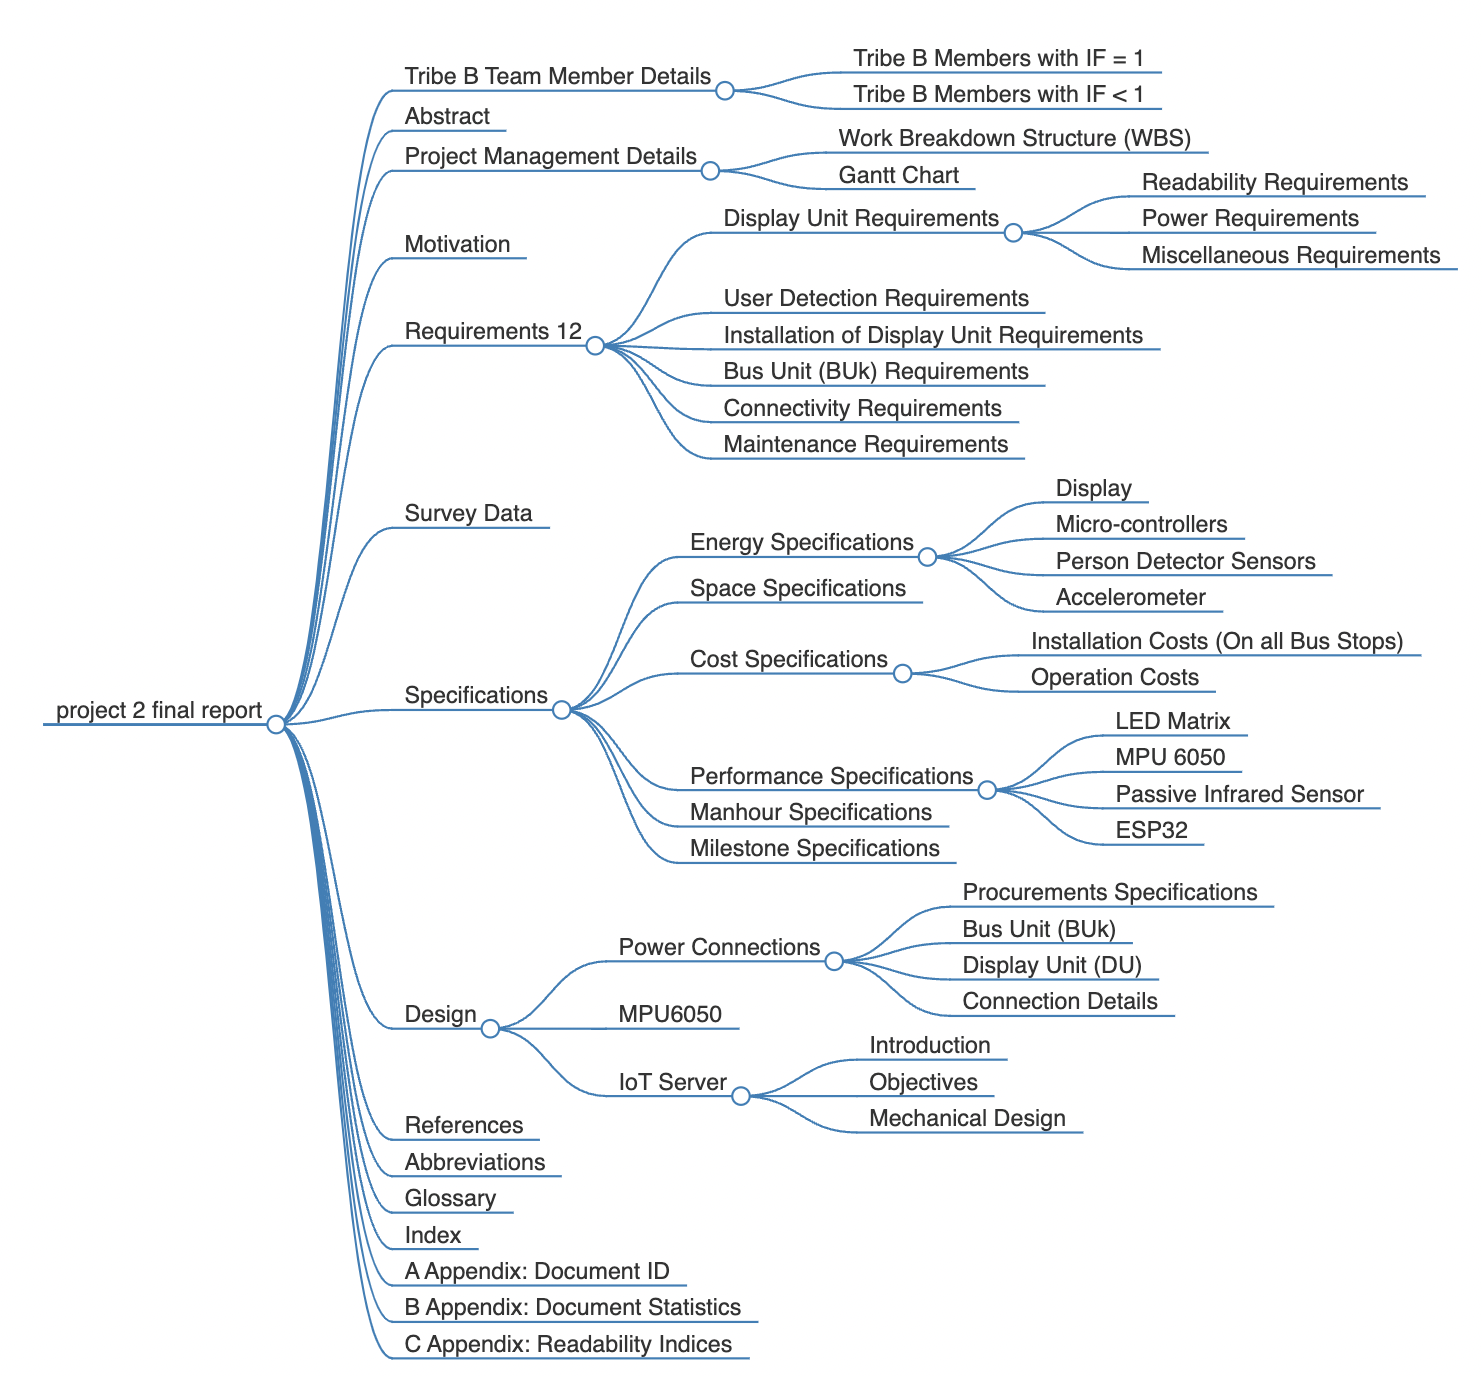
\includegraphics[scale=0.7]{mindmap.png}
\caption{Document Outline Mindmap}
    \label{fig:enter-label}
\end{sidewaysfigure}

\clearpage

\begin{abstract}
\addcontentsline{toc}{section}{\protect\numberline{}Abstract}
   This project aims to address the need for real-time bus arrival information at designated stops within the IITD campus. Presently operating with two buses, serving endpoints at the East Campus Market and DMS TIFAC Building. However, buses lack visible labels, leading to uncertainty among waiting passengers regarding the next available bus. To alleviate this issue, a comprehensive solution incorporating display units at bus stops and bus-mounted units (BUk) has been proposed. These units provide bilingual information on the estimated arrival time of the next bus and the operational status of each bus, ensuring transparency and facilitating informed commuting decisions. The system's design encompasses considerations such as readability, connectivity, power management, and weather resilience, essential for seamless operation under diverse conditions. Furthermore, data logging capabilities enable performance monitoring and maintenance scheduling, ensuring sustained operational efficiency. Through the integration of advanced technologies and robust infrastructure, this project endeavors to optimize campus transportation, enhancing user experience and fostering a more reliable and intuitive commuting environment.
    
\end{abstract}

\clearpage

\vspace{1cm}

\clearpage


\section{Project Management Details}

\subsection{\acrfull{WBS}}
A \acrshort{WBS} is a project management system that breaks projects into smaller, more manageable components or tasks. It is a visual tool that breaks down the entire project to make it easier to plan, organize, and track progress and assigns each task a unique identifier and places them within a hierarchical structure that shows the relationship between each task and its related deliverables.


\begin{figure}[h!]
\centering
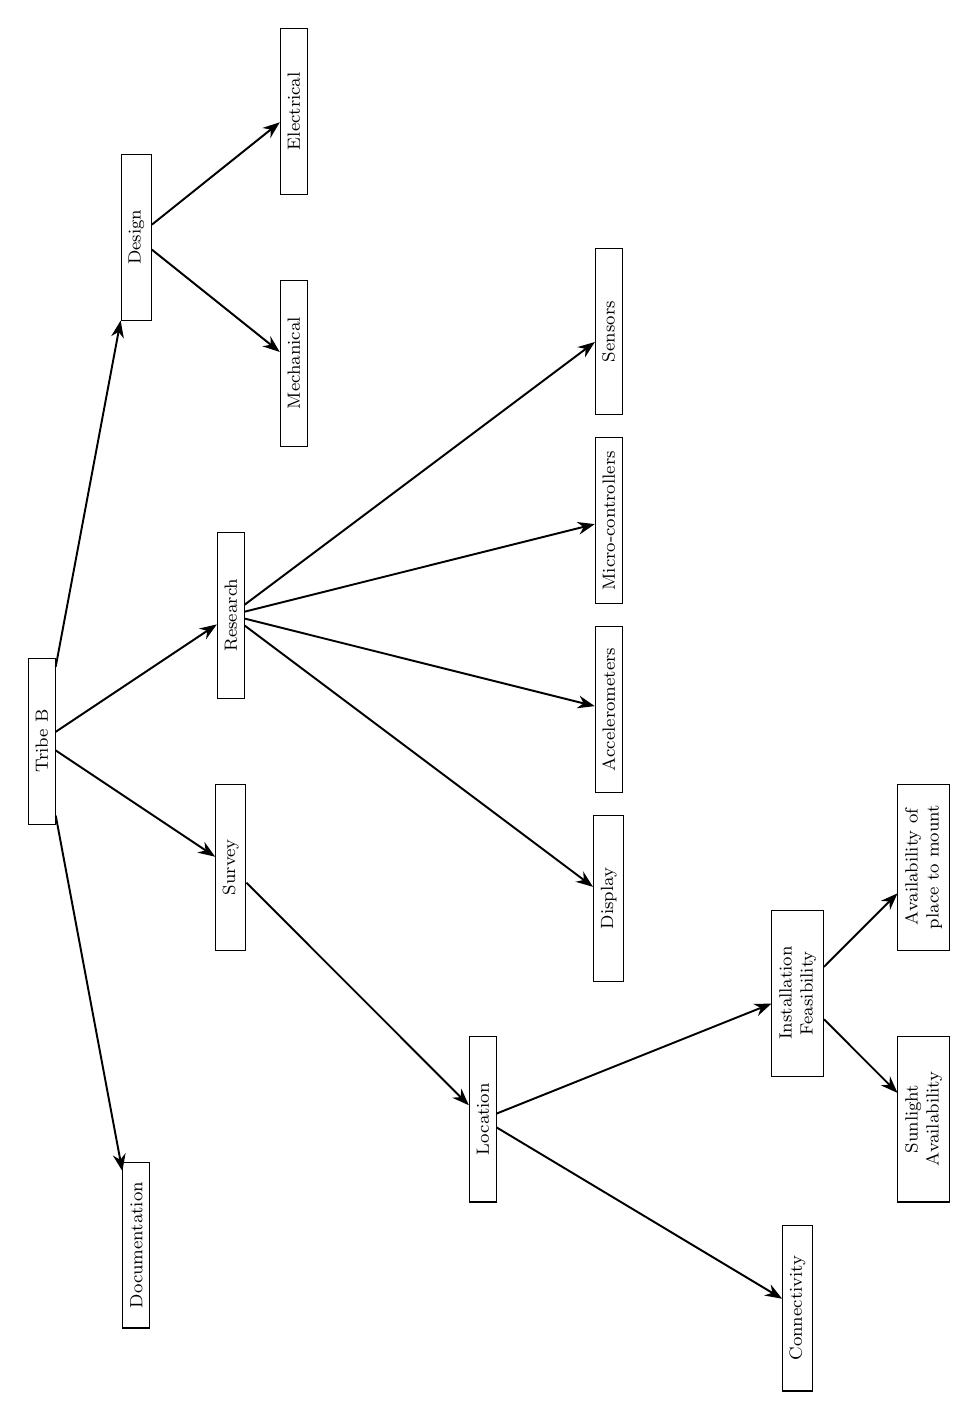
\begin{tikzpicture}[rotate=90, xscale=0.8, yscale=0.8,transform shape]
% Hey! Is this the new report?  Hello, anyone editing this document? 
\begin{scope}[every node/.style={shape=rectangle,
    draw, align=center,
    top color=white, bottom color=white!20,font = \footnotesize,text width=24mm},
    line/.style={draw, -latex'}]
    \node (a) at (0,0) {Tribe B};
    \node (b) at (-2,-3) {Survey};
    \node (c) at (-8,-1.5) {Documentation};
    \node (d) at (8,-1.5) {Design};
    \node (e) at (-6,-7) {Location};
    \node (f) at (2,-3) {Research};
\end{scope}

\begin{scope}[every node/.style={shape=rectangle,
    draw, align=center,
    top color=white, bottom color=white!20},
    line/.style={draw, -latex'},font = \footnotesize,text width=24mm]
    \node (g) at (3.5,-9) {Micro-controllers};
    \node (h) at (0.5,-9) {Accelerometers};
    \node (i) at (-2.5,-9) {Display};
    \node (k) at (6.5,-9) {Sensors};
    \node (l) at (-4,-12) {Installation Feasibility};   
    \node (r) at (-9,-12) {Connectivity};
    \node (y) at (10,-4) {Electrical};
    \node (z) at (6,-4) {Mechanical};
    \node (v) at (-6,-14) {Sunlight Availability};
    \node (w) at (-2,-14) {Availability of place to mount};
\end{scope}

\begin{scope}[
              every node/.style={fill=none,circle,black},
              every edge/.style={-Stealth,draw, line width=.7pt},
			  z/.style={line width=4pt,blue!40!cyan}  
              ]
    \path [-] (a) edge node[] {} (b); 
    \path [-] (a) edge node[] {} (f); 
    \path [-] (a) edge node[] {} (c); 
    \path [-] (a) edge node[] {} (d); 
    \path [-] (b) edge node[] {} (e); 
    
    \path [-] (f) edge node[] {} (k); 
    
    \path [-] (f) edge node[] {} (i); 
    \path [-] (f) edge node[] {} (h); 
    \path [-] (f) edge node[] {} (g); 
    \path [-] (e) edge node[] {} (l); 
    \path [-] (e) edge node[] {} (r); 
    \path [-] (d) edge node[] {} (z); 
    \path [-] (d) edge node[] {} (y); 
    \path [-] (l) edge node[] {} (v); 
    \path [-] (l) edge node[] {} (w); 
\end{scope}
\end{tikzpicture}
\caption{\acrshort{WBS}}
\end{figure}



\clearpage

\subsection{\index{Gantt Chart}{Gantt Chart}}
A Gantt chart is a type of bar chart that illustrates a project schedule. It lists the tasks to be performed on the vertical axis, and time intervals on the horizontal axis. The width of the horizontal bars in the graph shows the duration of each activity alongwith the start and finish dates of the terminal elements and summary elements of a project. It also shows the dependency relationships between activities.

\begin{figure}[H]
    \centering
    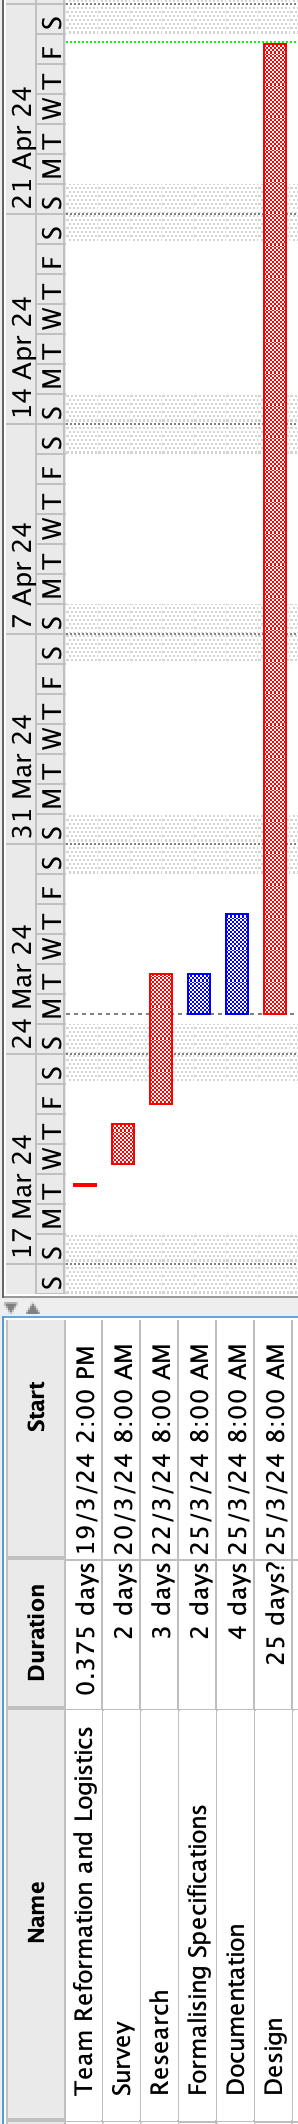
\includegraphics[width=0.15\textwidth]{gantt1.png}
    \caption{Gantt Chart}
    \label{fig:enter-label}
\end{figure}

\clearpage

    \section{Motivation}

Efficient transportation infrastructure is paramount within educational campuses, ensuring smooth mobility for students, faculty, and staff. However, existing intra-campus bus systems often lack essential features such as real-time arrival information\cite{gogri_real_nodate}, leading to inconvenience and uncertainty among commuters. This project aims to bridge this gap by addressing the pressing need for accurate and timely bus arrival information at designated stops within the campus.

The lack of visible labels on buses, coupled with staggered starting times, exacerbates the challenge for waiting passengers to predict the next available bus. Consequently, commuters face difficulties in planning their journeys effectively, leading to potential delays and frustration. By providing a comprehensive solution incorporating display units at bus stops and bus-mounted units (BUk), this project seeks to enhance the accessibility and reliability of campus transportation.

A review of existing literature underscores the significance of real-time transportation information in improving commuter satisfaction and overall system efficiency.Access to timely bus arrival information reduces perceived wait times, enhances commuter experience, and promotes the use of public transportation.

Furthermore, the integration of advanced technologies such as sensors for passenger detection, communication algorithms leveraging Bluetooth\index{Bluetooth} and WiFi\index{WiFi} protocols, and innovative display algorithms underscores the project's commitment to addressing contemporary challenges in campus transportation.

Through interdisciplinary collaboration and meticulous attention to design and functionality, this project endeavors to revolutionize campus transportation, fostering a more seamless and user-centric commuting experience for all stakeholders. By providing real-time bus arrival information, the system aims to optimize travel planning, reduce congestion, and promote sustainability within the campus environment. Ultimately, the motivation behind this research lies in enhancing the quality of life for campus residents and fostering a more efficient and reliable and intuitive transportation ecosystem.

\clearpage

\section{Requirements}
\subsection{Display Unit Requirements}
A display unit\index{display unit} must be installed at every bus stop that gives the waiting passengers an idea of the time it will take for the next bus to arrive.
    \subsubsection{Readability Requirements}
    \begin{enumerate}
        \item  The italicized portion of the display may be pre-printed with only the actual time displayed in flashing/blinking mode. \acrshort{lcd} displays with yellow back lighting can be used.
        \item  The display\index{display} must be readable by a person with 6/6 vision standing at any point within 8 feet in front of the bus stop. 
        \item The display has to read 999 in case of any emergencies or unforeseen delays.
    \end{enumerate}
    \subsubsection{Power Requirements}
    \begin{enumerate}
        \item The display unit in the stop must be battery powered and must work between 0700 and 1930 hours. 
        \item Outside these hours, it must self-power down and auto-restart the next day. 
        \item Solar power must be provided as an option. (Since bus stops are generally located in the shade, suitable nearest sun point has to be found for usage of solar power)
    \end{enumerate}
    \subsubsection{Miscellaneous Requirements}
    \begin{enumerate}
        \item The reading on the display must be accurate to ±1 minute. 
        \item The Bus Stop unit has a white downward pointing \acrshort{led} which blinks with a 30\% duty cycle during normal service. 
        \item In case of any unforeseen malfunction in the display unit, a stall period of 1 hour will be allowed to fix the issue. 
    \end{enumerate}
    
\subsection{User Detection Requirements}
        The presence of a waiting passenger standing for more than 30 seconds in any stop may optionally trigger a detector, and be used to inform (the single bicolor \acrshort{led} in the {\acrshort{buk}} starts blinking) the bus unit \acrshort{buk} that passengers are waiting. The passenger is detected automatically. 
        
\subsection{Installation of Display Unit Requirements}
\begin{enumerate}
    \item \gls{IP67}\index{IP67} enclosures are to be used and will be provided by the lab. Four enclosures per Tribe for the DU unit will be provided - two to be used for the Route 1 bus stops and two for the other Route 2.
    \item The display units should be difficult to steal and sell, this is to be ensured with mechanical fixation and placing it at an unreachable height.
\end{enumerate}

\subsection{Bus Unit (BUk) Requirements}
\begin{enumerate}
    \item It is mandatory for each bus to have a separate Bus Unit (BUk) (the ‘k’ in BUk refers to the kth bus).
    \item The BUk must contain one bi-colour \acrshort{led} which can switch between red and green.
    \item The colours that the unit display will follow the following protocol:
    \begin{enumerate}
        \item A red colour will indicate that the bus is out of service, and every stop on the route will display a suitable warning for waiting passengers. 
        \item A red \acrshort{led} which is also blinking is another combination, that is open to be used for flagging specific errors in design.
        \item A green \acrshort{led} implies that the bus is functioning normally.
        \item A green \acrshort{led} which is also blinking means that the passengers are waiting at at least one of the bust stops on the route.
        \item Apart from this, a white \acrshort{led} is also available for use, but is up to the vendors’ discretion. 
    \end{enumerate}
    \item The BUk\index{BUk} is powered from the battery of the bus (primary power) and from a separate internal battery (secondary power). Primary power is available whenever the ignition is on or the when the engine has started. Secondary power is on at all remaining times. Switchover from primary to secondary power is automatic and without human intervention. A BUk cannot be turned off. 
    \item The BUk has a red toggle switch with positions 1 and 2 - pressing it to position 1 means that the bus is out of service.
    \item The BUk is expected to be as compact as possible, and is to be placed on the dashboard of the bus along with the toggle button.
    \item The BUk is also expected to keep the bus activity and travel logs for the past month.
\end{enumerate}

\subsection{Connectivity Requirements}
    \begin{enumerate}
        \item Non-availability of cellular connectivity (like WiFi or \acrshort{gsm}) should not interrupt the working of the system.
        \item Occasional use of WiFi\index{WiFi} (IITD WiFi) is allowed.
        \item The use of Bluetooth \acrshort{ble} is allowed in both BUk and the Display Units. 
        \item Any form of connectivity \index{connectivity} (wireless or wireless) which is legally allowed in India is allowed.
    \end{enumerate}
    
\subsection{Maintenance Requirements}
\begin{enumerate}
    \item A digital interface to collect feedback \index{feedback} from users and to allow the users to report errors is to be implemented. 
    \item Resources to perform daily maintenance of the display units and the bus units are available.  
    \item Metrics like logging start times, times at which the bus reach each stop and left that bus stop, and duration of out-of-service will be used as base metrics to evaluate efficiency and reliability of the bus service. 
\end{enumerate}



\clearpage

\section{Survey Data}
\begin{table}[h!]
\centering
\begin{tabular}{|c|c|c|c|c|}
\hline
S. No. & Bus Stop Location & Latitude(\degree N) & Longitude(\degree E) & IITD Wifi Strength (dbm) \\
\hline
1 & Shivalik & 28.5480 & 77.1856 & -65 \\
2 & Kailash &28.5442 &77.1957 &-78 \\
3 & Market &28.5428 &77.1990 &-65 \\
4 & Kumaon &28.5491 &77.1849 &-74 \\
5 & Aravali &28.5483 &77.1840 &-65 \\
6 & Karakoram &28.5473 &77.1834 &-75 \\
7 & Central Workshop &28.5441 &77.1921 &-70 \\
8 & Main building &28.5444 &77.1928 &-65 \\
9 & Bharti school &28.5448 &77.1899 &-73 \\
10 & IIT Hostpital &28.5455 &77.1882 &Poor connection \\
11 & Nilgiri &28.5461 &77.1829 &-71 \\
12 & DMS &28.5428 &77.1824 &Poor connection \\
13 & Rajdhani &28.5460 &77.1868 &Poor connection\\
14 & Kalyan Mandap &28.5409 &77.1981 &Not Available\\
15 & B-15 Gate 3 &28.5404 &77.1973 &Not Available\\
16 & Block B-18 &28.5408 &77.1961 &Not Available\\
17 & B-12 Bus Stop &28.5413 &77.1951 &Not Available\\
\hline
\end{tabular}
\caption{Bus Stop Data}
\label{tab:teamDetails}
\end{table}
As part of the survey team tasked with evaluating the feasibility of installing WiFi\index{WiFi} hotspots\index{hotspots} powered by solar panels at various bus stops within the IIT Delhi campus, we conducted a thorough assessment of each stop's geographical coordinates, WiFi signal strength, and potential installation challenges. Our findings indicate a range of scenarios across the surveyed bus stops.

\\Starting with Shivalik, situated at latitude\index{latitude} 28.54797 and longitude\index{longitude} 77.18564, the WiFi signal strength was measured at 65 dBm. However, due to limitations in solar panel installation, alternative locations for WiFi deployment were explored, with the nearest viable option identified as the SAC circle.

\\Moving on to Kailash, located at latitude 28.5441928 and longitude 77.1957229, the WiFi signal strength was significantly lower at -78 dBm. Similar to Shivalik, solar panel installation was deemed impractical. The Himadri circle emerged as a potential alternative location for WiFi deployment.

\\In contrast, IIT Market and Kumaon exhibited stronger WiFi signal strengths at -65 dBm and -74 dBm, respectively, rendering them suitable for solar panel installation. For Kailash Market, the identified installation spot was supported by adjacent solar exposure, while Kumaon's alternative location lay on the opposite side of the stop.

\\Additionally, stops such as Aravali, Karakoram, and the main building boasted favorable WiFi signal strengths, allowing for solar panel installation. These stops presented opportunities for enhancing connectivity within the campus environment.

\\However, challenges were encountered at Central Workshop, where WiFi signal strength was suboptimal, and solar panel installation was unfeasible. Similarly, Nilgiri and Rajdhani/Yulu Bike Zone displayed poor WiFi connectivity, limiting installation options. The nearest place for wifi installation for Rajdhani stop is SAC circle or Apollo pharmacy. DMS stop exhibit poor connection but solar battery can be installed.
\\Furthermore,  assessment of stops near girls hostel :
\\Kalyan Mandap: Despite no steel pole availability, sunlight exposure within the premises offers potential for alternative power sources. Local WiFi networks are operational, providing connectivity options.
\\B15 Gate 3: With a steel pole available and sunlight exposure, this stop offers favorable conditions for solar panel installation. Local WiFi networks contribute to connectivity options.
\\Block B-18: Although lacking a steel pole, the presence of a nearby pole offers a mounting solution. Sunlight exposure and operational local WiFi networks enhance feasibility.
\\B-12 Bus Stop: Featuring a steel pole and sunlight exposure, this stop presents ideal conditions for solar panel installation. Operational local WiFi networks contribute to connectivity options.
\\For above four stops. IITD WiFi seemed not to be working, but local blocks wifi were available and connection to these local WiFi could not be made to measure their strength.
\\Photographic evidence was provided for each bus stop, facilitating visual inspection of site conditions and potential installation challenges.
Based on the survey findings, recommendations were made regarding suitable locations for WiFi hotspot installation, considering factors like WiFi signal strength, sunlight exposure, and availability of steel poles for mounting solar panels.

\clearpage

\section{Specifications}
\subsection{Energy Specifications}
\subsubsection{Display}
\begin{itemize}
    \item We will use the 8x8 dot \acrshort{led} matrix, which is highly efficient for the display in the project.
    \item Forward Voltage: 2.1V $\approx$ 2.5V
    \item Forward Current: 20mA
    \item The power consumption per \acrshort{led} can be calculated as P = IV, where P is power in watts, I is current in amperes, and V is voltage in volts. For a 3.3V supply and a forward current of 20mA, the power consumption per \acrshort{led} would be P = 0.02A $\times$ 3.3V = 0.066W or 66mW. For the entire display, this would be 64 $\times$ 0.066W = 4.264W.
    \item The display has to work from 07:00 to 19:30.
    \item There are 17 stops, each with a display.
    \item Therefore, the maximum energy requirement per day = 4.264$\times$12.5$\times$17 = 0.906 kWh

\end{itemize}

\subsubsection{Micro-controllers}
\begin{itemize}
    \item We will be using ESP32 \index{ESP32} Dev Boards
    \item 4 ESP32-Dev boards will be powered by USB cables and a power bank.
    \item The ESP32 board can draw up to 600mA during peak operations, and the typical operating voltage is 3.3 V with support for external power with an input voltage range of 5V-9V, which is regulated onboard.
    \item These boards will operate continuously for 24 hours.
    \item Therefore, the estimated daily energy requirement = 3.3$\times$0.6$\times$24$\times$4 = 0.19 kWh

\end{itemize}

\subsubsection{Person Detector Sensors}
\begin{itemize}
    \item Passive Infrared sensors will be installed on all 17 bus stops
    \item \acrfull{pir} sensors typically operate on a voltage range of 5V to 20V
    \item The power consumption of \acrshort{pir}\index{PIR} sensors is relatively low, with a power consumption of 65 mA at 5V
    \item \acrshort{pir} sensors will work from 07:00 to 19:30
    \item Therefore, average daily energy requirement = 0.065$\times$5$\times$12.5$\times$17 = 0.069 kWh

\end{itemize}

\subsubsection{\gls{Accelerometer}}
\begin{itemize}
    \item 2 accelerometers\index{accelerometers} will be used, one in each BUk unit. The part number of one of these units is \gls{MPU 6050}
    \item They will draw power indirectly via the ESP32 Board. They will operate via the provided power bank when on secondary power and directly from the bus battery when on primary power. They will power down when the bus is not in business hours
    \item The Voltage requirement of the device is 5 V, and the max current intake of the device is 3.9 mA
    \item The device will be on during business hours from 07:00 to 19:30, which is 12.5 hours
    \item Therefore, the estimated daily energy requirement = 5$\times$3.9$\times$0.001$\times$12.5$\times$2 = 0.4875 Wh $\approx$ 0.0005 kWh

\end{itemize}
\subsection{Space Specifications}
\begin{itemize}
    \item \textbf{ Enclosures}
    \begin{enumerate}
    \item Display Units (DU)
    \begin{itemize}
      \item Dimension - 27.5cm $\times$ 27.5cm $\times$ 10.5cm
    \end{itemize}
    
    \item Bus Units (BU)
    \begin{itemize}
      \item Dimension - 15cm $\times$ 12cm $\times$ 8cm
    \end{itemize}
    \end {enumerate}

    \item \textbf{Solar Panel}
    \begin{itemize}
        \item Active Panel Area - 30cm $\times$ 21.5cm
        \item Total Area - 25.5cm $\times$ 35cm
    \end{itemize}
    
    \item \textbf{Wires}
        \begin{itemize}
            \item  The wires are noted to have a minimal spatial impact, as they are either positioned underground or closely attached to the steel pole.
        \end{itemize}
    
\end{itemize}

\subsection{Cost Specifications}
\subsubsection{Installation Costs (On all Bus Stops)}
\begin{itemize}
    \item Display Unit\index{Display Unit}
    \begin{enumerate}
        \item Cost of Single Unit = 144 INR
        \item Number of Units Required = 17 + 3 (Spare)
        \item Total Cost = 2880 INR
    \end{enumerate}
    \item \gls{ESP32} Dev Board + Connecting Cable
    \begin{enumerate}
        \item Cost of Single Unit = 500 INR
        \item Number of Units Required = 4
        \item Total Cost = 2000 INR
    \end{enumerate}
    \item \gls{Accelerometer}
    \begin{enumerate}
        \item Cost of Single Unit = 101 INR
        \item Number of Units Required = 2
        \item Total Cost = 202 INR
    \end{enumerate}
    \item PIR Sensors
    \begin{enumerate}
        \item Cost of Single Unit = 150 INR
        \item Number of Units Required = 17 + 3(Spare)
        \item Total Cost = 3000 INR
    \end{enumerate}
    \item Solar Panels
    \begin{enumerate}
        \item Cost of Single Unit = 900 INR
        \item Number of Units Required = 17 + 1(Spare)
        \item Total Cost = 16200 INR
    \end{enumerate}
    \item Solar Charge Convertor\cite{technology_pwm_2021}
    \begin{enumerate}
        \item Cost of Single Unit = 200 INR
        \item Number of Units Required = 17 + 1(Spare)
        \item Total Cost = 3600 INR
    \end{enumerate}
    \item DC-DC 12-5 Volts Converter\cite{noauthor_dc_nodate}
    \begin{enumerate}
        \item Cost of Single Unit = 100 INR
        \item Number of Units Required = 2
        \item Total Cost = 200 INR
    \end{enumerate}
    \item Wire
    \begin{enumerate}
        \item Cost per m = 15 INR
        \item Length Required = 20
        \item Total Cost = 300 INR
    \end{enumerate}
    \item Enclosures
    \begin{enumerate}
        \item Cost per unit = 200 INR
        \item Number of Units required = 17 + 2 + 3(Spare)
        \item Total Cost = 4400 INR
    \end{enumerate}
\end{itemize} 
\subsubsection{Operation Costs}
\begin{itemize}
    \item The devices are self sufficient. They are powered via solar panels
    \item The only operation cost is the maintenance of the devices and the maintenance of the database, which is minimal compared to the installation cost.
\end{itemize}

\subsection{Performance Specifications}
\subsubsection{\acrshort{led} Matrix}
The red colour emitted by the LEDs\cite{noauthor_-depth_2020} is chosen for its visibility in low-light conditions. The contrast between the black background of the display and the red LEDs helps in making the display content stand out, making it easier to read . The forward current of 20mA is sufficient to ensure the LEDs are bright enough to be readable from a distance of 8 feet. The operating temperature range of the device is 40 to 85°C which ensures that the display can be used in a wide range of environments, including those with varying temperatures\index{temperatures}.

\subsubsection{\gls{MPU 6050}}
The \gls{MPU 6050}\cite{noauthor_arduino_2021} supports I2C communications\cite{noauthor_basics_nodate} at up to 400kHz. Given you use 400kHz I2C speed, the highest data rate to read all values is theoretically 2.61kHz, 2.96kHz if you omit the temperature reading (15 bytes must be transmitted, needing 9 clocks each). The \gls{MPU 6050} can have a sample rate of 1 KHz if you are able to read values out at that speed. It will be difficult if you are reading every gyro and accel every time and you are using I2C. Your MPU allows a sample rate of 8kHz only for the \gls{gyrometer}, the accelerometer allows only 1kHz.

\subsubsection{\acrlong{pir} }
Human bodies typically radiate infrared\index{infrared} energy concentrated in the wavelength range of 8 um-12 um.The sensor detects infrared radiation from the human body, triggering an alarm.
\begin{itemize}
    \item Field of View: Narrow field of view, typically around 90 to 180 degrees.
    \item Input/Output Type: Digital output indicating motion detection \index{motion detection}.
    \item Range: Typically up to 10 meters.
    \item Changes in Weather: \acrshort{pir}\cite{noauthor_passive_nodate} sensors may be affected by temperature changes, especially extreme variations between summer and winter.
    \item Day Switches\index{Day Switches}: Can be affected by changes in ambient light levels, such as transitioning from noon to evening.
    \item Price: Generally affordable.
    \item Ease of Use: Easy to install and set up.
    \item Needs An optical system, including a plastic Fresnel lens\index{Fresnel lens}, focuses infrared radiation onto the pyroelectric sensor\index{pyroelectric sensor} to enhance detection distance.
\end{itemize}

\subsubsection{\gls{ESP32}}
The ESP32\cite{noauthor_introduction_nodate} is a series of low-cost, low-power system-on-chip microcontrollers. It is designed and manufactured by Espressif Systems.
It is a successor to ESP8266 SoC and comes in single-core and dual-core variations of the Tensilica’s 32-bit Xtensa LX6 Microprocessor with integrated Wi-Fi and Bluetooth. Its integrated RF components include Power Amplifier, Low-Noise Receive Amplifier, Antenna Switch, Filters and RF Balun. This makes designing hardware around ESP32 very easy as you require very few external components.
Some of its Specifications are-

\begin{itemize}
    \item Single or Dual-Core 32-bit LX6 Microprocessor with clock frequency up to 240 MHz
    \item 520 KB of SRAM, 448 KB of ROM and 16 KB of RTC SRAM.
    \item Supports 802.11 b/g/n Wi-Fi connectivity with speeds up to 150 Mbps.
    \item Support for both Classic Bluetooth v4.2 and BLE specifications.
    \item 34 Programmable GPIOs.
    \item Up to 18 channels of 12-bit SAR ADC and 2 channels of 8-bit DAC
    \item Serial Connectivity include 4 x SPI, 2 x I2C, 2 x I2S, 3 x UART.
    \item Ethernet MAC for physical LAN Communication (requires external PHY).
    \item 1 Host controller for SD/SDIO/MMC and 1 Slave controller for SDIO/SPI.
    \item Motor \acrshort{PWM} and up to 16-channels of LED \acrshort{PWM}.
    \item Secure Boot and Flash Encryption.
    \item Cryptographic Hardware Acceleration for AES, Hash (SHA-2), RSA, ECC and RNG.
\end{itemize}

\subsection{Manhour Specifications}
\begin{itemize}
    \item Estimate of Man-Hours in Development of Product
\\45 (Persons on Team) $\times$ 10 (Hours per member) = 450 
\item Estimate of Man-Hours in Installations
\\17 Stops $\times$ 2 hours per stop = 54 hours
\item Estimate of Man-Hours in Maintenance 
\\ Once every month for 17 stops $\times$ 15 mins per stop = 5 hours/month
\end{itemize}


\clearpage

\subsection{Milestone Specifications} 

\begin{table}[H]
\begin{tabularx}{\textwidth}{|c|X|X|r|c|} 
\hline
Milestone & Description & Division & Marks & \acrshort{TRL} \\
\hline
\multirow{6}{3.8em}{1} & \multirow{6}{9em}{Survey} & Decision of what to be collected and Methodology & 6 & \multirow{6}{3em}{\acrshort{TRL}-1} \\
& & Collecting of data near girls hostel & 6 & \\ 
& & Collecting of data near boys hostel & 6 & \\ 
& & Collecting of data near Amul and insti area & 6 & \\ 
\hline
\multirow{6}{3.8em}{2} & \multirow{6}{9em}{Design of Algorithm} & Design of suitable logging mechanism & 6 & \multirow{6}{3em}{\acrshort{TRL}-2}\\ 
& & Design of suitable Communication Protocol & 6 & \\ 
& & Design of suitable protocol for Display of bus timings & 6 & \\ 
& & Contingencies in case of a Wi-fi failure & 6 & \\ 
\hline
\multirow{6}{3.8em}{3} & \multirow{6}{9em}{Model Design} & Implementation of basic communication between modules(Wifi and Bluetooth deployment) & 6 & \multirow{6}{3em}{\acrshort{TRL}-3}\\ 
& & Circuit Design of BUk & 6 & \\ 
& & Circuit Design of DUk & 6 & \\ 
& & CAD Model of device & 6 & \\ 
\hline
\multirow{6}{3.8em}{4} & \multirow{6}{9em}{Final Demonstration} & Logging of Data  & 7 & \multirow{6}{3em}{\acrshort{TRL}-4}\\ 
& & Communication between BUk and DUk & 7 & \\ 
& & Communication between BUk and Wi-Fi & 7 & \\ 
& & Display of Timings on device & 7 & \\ 
\hline
\end{tabularx}
\caption{Milestone \acrshort{TRL}}
    \label{tab:Milestone Specifications}
\end{table}

\clearpage
\section{Design}
\subsection{Power Connections}
\subsubsection{Items to Procure and Specifications}
\begin{enumerate}
    \item Enclosures for BUk and DUk
    \item Solar panels (10W/6A)
    \begin{enumerate}
        \item  Open Circuit Voltage 21.7V
        \item SC Current 600mA
        \item Product Dimensions = $30L \times 34W \times 1.7H cm$
        \item Connector Type = 14AWG
        \item Maximum Voltage = 12 Volts
        \item Maximum Power	= 10 Watts
    \end{enumerate}
    \item \acrshort{PWM} Solar Charge Converters: Solar charge controllers are used to regulate the power coming from solar cells. These charge controllers can not only power devices directly but can also charge the backup batteries. They also keep the batteries safe from overcharging. 
    \begin{enumerate}
        \item Voltage 24 Volts
        \item Works on 12 And 24 Volts both 06 Amp 100 Watt Solar Panel Max.
        \item Product Dimensions = $13.5 \times 9 \times 4 cm$; 180 Grams
        \item ASIN	B07MVN922P
    \end{enumerate}
    \item USB cables
    \item ESP32 S-series Voltage: 3.3 V
    \item Rechargeable Battery: It will store solar energy and provide power during periods of low sunlight.
    \item DC-DC buck converters (12V stepped down to 5V)
\end{enumerate}
\subsubsection{Bus Unit (BUk)}
\begin{enumerate}
    \item \textbf{Primary Power} The BUk will receive primary power directly from the bus battery (12V nominal) through the USB output on the panel.
    \item \textbf{Secondary Power} A separate internal battery will provide secondary power when the bus engine is off.
\end{enumerate}
The switching between them is taken care of by a relay switch in the Main Model.

\begin{figure}[H]
    \centering
    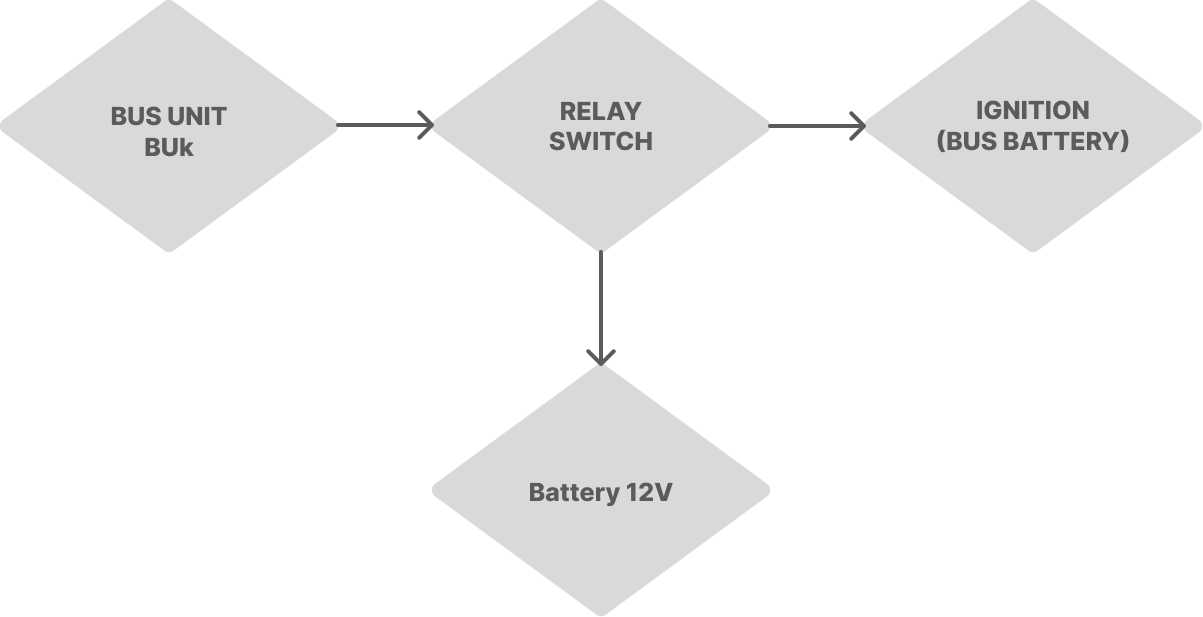
\includegraphics[width=0.8\textwidth]{Group 456.png}
    \caption{Main Model}
    \label{fig:enter-label}
\end{figure}
\subsubsection{Display Unit (DU)}
\begin{enumerate}
    \item \textbf{Primary Power} A rechargeable battery will be the primary power source for the DU.
    \item \textbf{Secondary Power} 
    \begin{enumerate}
        \item A 10W/6A solar panel connected through a \acrshort{PWM} Solar Charge Converter will provide secondary power and charge the battery.
        \item The \acrshort{PWM} Solar Charge Converter ensures efficient battery charging based on solar panel output.
    \end{enumerate}
\end{enumerate}
\subsubsection{Connection Details}
DC-DC buck converters typically have labeled terminals for solar panel input, battery connection, and output voltage (3.3V for the buck converter).
\begin{enumerate}
    \item \textbf{Solar Panel:} The positive and negative terminals of the solar panel are connected to the corresponding terminals on the \acrshort{PWM} solar charge controller (usually labeled "PV+" and "PV-").
    \item \textbf{Battery:} The battery's positive and negative terminals are connected to the designated battery terminals on the \acrshort{PWM} solar charge controller (usually labeled "BAT+" and "BAT-").
    \item \textbf{DC-DC Buck Converter:} The battery's positive terminal is connected to the DC-DC buck converter's input voltage terminal (usually labeled "Vin"). The converter's ground terminal is then connected to the battery's negative terminal. The ESP32's Vin power pin is conneced to the DC-DC buck converter's output voltage terminaland the ESP32's ground pin is connected to the converter's ground terminal.
\end{enumerate}
\textbf{Location of Solar Panel} could be at the top of the Bus Stop pole, which has a frame for supporting it and receives sufficient sunlight.
The surveyed wire length required is around \textbf{20 inches} from the top to the timetable board. 

\begin{figure}[H]
    \centering
    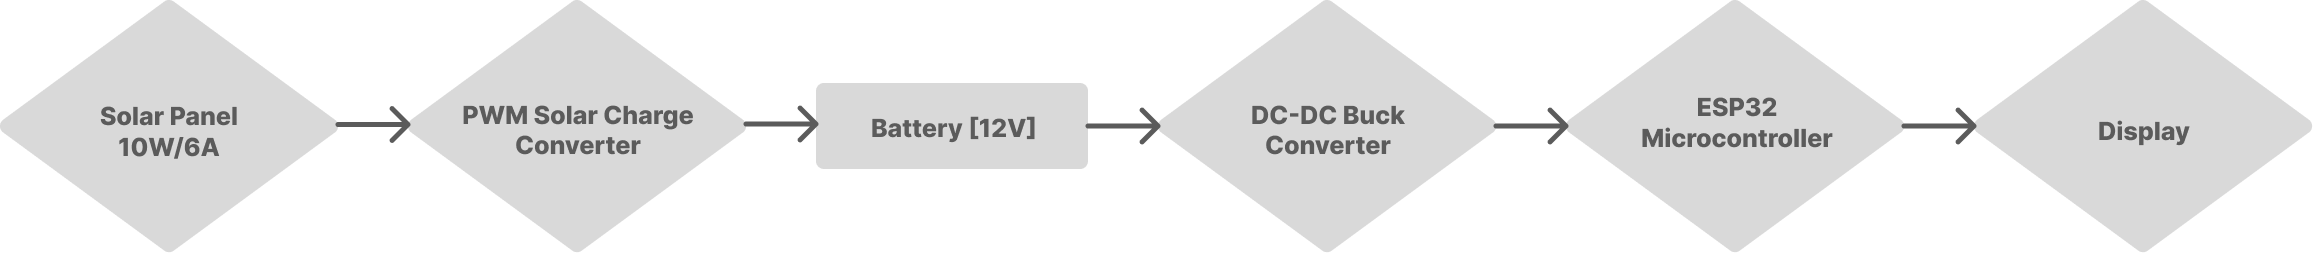
\includegraphics[width=1\textwidth]{Group 462.png}
    \caption{Diagram of Connections}
    \label{fig:enter-label}
\end{figure}


\subsection{MPU6050}
Arduino codes were simulated on Wokwi and then tested on ESP32 separately for
mpu and LED as well as after integration.
\vspace{10pt}
\\Normally the velocity would be calculated from the acceleration values, which
would help us determine the state of motion. However, there is always a small
error in the acceleration values which leads to a huge error in the velocity
calculation. Hence, we use the acceleration values alone - assuming that the bus
cannot be in motion with constant velocity (0 acceleration) beyond a fixed time
limit except during rest (in this case, we have taken the fixed time to be 5
seconds). Therefore the bus would be perceived to be at rest only when the
acceleration is 0 for more than 5 seconds.
We have added all the components of the acceleration and set a limit of $10.2 m/s^2$ which is a little above the acceleration due to gravity. If the
resultant acceleration crosses this limit the bus would be perceived to be in
motion.
Finally, by the procedure mentioned above, it can be determined if the bus is at
rest at the stop and this information can be relayed further.

\subsection{IoT Server}

\subsubsection{Introduction}
The project involved creating an IoT system utilizing an ESP32 device to transmit data to an IoT server. The server, built on the ThingSpeak platform by MathWorks, was designed to receive, analyze, and display real-time data from the ESP32 device. The primary goal was to establish a seamless connection between the ESP32 device and the ThingSpeak server to enable efficient data monitoring and visualization.

\subsubsection{Objectives}
\begin{enumerate}
    \item Establish a stable connection between the ESP32 device and the ThingSpeak server.
    \item Implement data transmission protocols to send relevant data from the ESP32 to the server. 3. Develop a user interface on ThingSpeak to visualize and analyze the incoming data streams. 4. Ensure scalability and reliability of the IoT system for future expansion and integration.
\end{enumerate}


\subsubsection{Methodology}
\begin{enumerate}
    \item Hardware Setup: Utilized an ESP32 device as the data transmitter, connected to various sensors or instruments for data collection.
    \item Software Development:
    \begin{itemize}
        \item Configured the ESP32 device to establish a connection with the local hotspot.
        \item Implemented data formatting and transmission protocols (e.g., MQTT, HTTP) for sending data to the ThingSpeak server.
        \item Created MATLAB scripts and code on ThingSpeak to receive, process, and display incoming data.
    \end{itemize}
    \item Integration and Testing:
    \begin{itemize}
        \item Integrated the ESP32 device with the ThingSpeak server to ensure seamless data transmission.
        \item Conducted extensive testing to verify the accuracy, reliability, and real-time nature of data displayed on the server.
    \end{itemize}
    \item User Interface Design:
    \begin{itemize}
        \item Designed a user-friendly interface on ThingSpeak to visualize data using plots, charts, and gauges.
        \item Implemented customization options for users to modify visualization parameters as needed.
    \end{itemize}
    \item Outcome: The successful implementation of the IoT system led to the following outcomes:
    \begin{itemize}
        \item Real-Time Data Monitoring: Users could monitor and analyze real-time data streams from the ESP32 device through the ThingSpeak server.
        \item Data Visualization: The user-friendly interface on ThingSpeak facilitated data visualization through plots, charts, and gauges, enabling better insights and decision-making.
    \end{itemize}
\end{enumerate}

\subsubsection{Mechanical Design}
We worked on designing how the bus stop enclosure would be fixed to the pole and how the dot matrix and lens structure would be held together.

\subsubsection{WiFi}
Wrote Arduino code using the following libraries: WiFi.h, Arduino.h, and used platform.io to connect to external WiFi, given the WiFi ID and password. Connected ESP32 (3.3 V) with USB cables to check if it is connected or not. 
We also deployed the code into ESP32 and checked the range of distance up to which it remains connected. If disconnected, the led is expected to start blinking and on being connected (or reconnected) to wifi on coming in its vicinity, the led light is expected to become consistent. The MAC address and IP Address were also obtained.
\clearpage
\subsection{Source Code}
\subsubsection{Code for Stop Unit A}
\begin{lstlisting}[style=myArduino]
#include "time.h"
#include <esp_now.h>
#include <WiFi.h>
#include <MD_Parola.h>
#include <MD_MAX72xx.h>
#include <SPI.h>


#define STOP_A  0
#define STOP_B  1
#define BUS  2

// Define hardware type, size, and output pins for 8*8 LED Display
#define HARDWARE_TYPE MD_MAX72XX::ICSTATION_HW
#define MAX_DEVICES 2
#define CS_PIN 5
#define DATA_PIN 19
#define CLK_PIN 18

// Motion Macros
#define MOVING 0
#define STOP_AT_A 1
#define STOP_AT_B 2
#define STOP_BETWEEN 3
#define MOTION_ACC 0
#define REST_ACC 1
#define ERR_VAL 4
#define TIME_OUT_FOR_MOTION_IN_MILLI 5000

// Out of Service Macros
#define INSERVICE 0
#define OUTOFSERIVCE 1

// Time of travel
#define INITIAL_TIME 60
#define TIME_FROM_A_TO_B 180 
#define TIME_FROM_B_TO_A 60
#define STOPTIME 60

// Delay Status
#define DELAYED 0
#define ONTIME 1

#define BUTTON_PIN 0 // GPIO21 pin connected to button

uint8_t motionStatus = MOVING;

// NTP Server and External Wifi Related Configurations:
const char* externalSSID =  "ELP305 P2";
const char* externalPassowrd = "Qwerty@123";  

const char* ntpServer = "time.google.com";
const long  gmtOffset_sec = 0;
const int   daylightOffset_sec = 19800;//GMT+5:30

// Starting time of all the devices.
const uint8_t Starthours = 16;
const uint8_t Startminutes = 10;

const int ownIdentity = STOP_A; // Identity = 0 for StopA, 1 for StopB, 2 for Bus Unit

uint8_t broadcastAddressStopA[] = {0xEC, 0x64, 0xC9, 0x86, 0x4C, 0x38};
uint8_t broadcastAddressStopB[] = {0x30, 0xC9, 0x22, 0x28, 0x4F, 0x60};
uint8_t broadcastAddressBusUnit[] = {0xEC, 0x64, 0xC9, 0x82, 0x7E, 0x34};

const char* ssidStopA  = "ESP32-Access-StopA";
const char* ssidStopB  = "ESP32-Access-StopB";
const char* ssidBusUnit = "ESP32-Access-BusUnit";

uint8_t running_timer = 60;
uint8_t delay_timer = 0;
uint8_t delayStatus = ONTIME;
uint8_t outofserviceStatus = OUTOFSERIVCE;

uint8_t passenger = 0;

float rssiA_B = 0.0;
// float rssiB = 0.0;

uint8_t inReadings[5];
bool valueRecieved = false;
uint8_t incomingAddr[6]; 

uint8_t outReadings[5];

esp_now_peer_info_t peerInfo1;
esp_now_peer_info_t peerInfo2;

esp_now_send_status_t lastPacketSendStatus = ESP_NOW_SEND_FAIL;

void OnDataSent(const uint8_t *mac_addr, esp_now_send_status_t status) {
  lastPacketSendStatus = status;
}

void OnDataRecv(const uint8_t * mac, const uint8_t *incomingData, int len) {
  memcpy(&inReadings, incomingData, sizeof(inReadings));
  memcpy(&incomingAddr, mac, sizeof(incomingAddr));
  valueRecieved = true;
}

hw_timer_t * timer = NULL;
volatile uint8_t count = 0; 
bool timerWork = false;

void IRAM_ATTR onTimer(){ // 8 instances. 1 to 8.
  running_timer = running_timer - 2;
  if(count < 8){
    count++;
    timerWork = true;
    return;
  }
  else{
    timerWork = true;
    count = 1;
  }
  return;
}

MD_Parola myDisplay = MD_Parola(HARDWARE_TYPE, DATA_PIN, CLK_PIN, CS_PIN, MAX_DEVICES);

// Used to print out of service message in case of failure
void displayOutOfService(){
  
  myDisplay.setIntensity(5);
  myDisplay.displayClear();
  myDisplay.displayText("Out of Service", PA_CENTER, 100, 0, PA_SCROLL_LEFT, PA_SCROLL_LEFT); //(Text, Letak, speed)
  Serial.println("OutOfSerive");

  if (myDisplay.displayAnimate()) {
    myDisplay.displayReset();
  }
}

// // Display Time on the 8*8 LED Matrix in minutes
void displayNumber(int num){
  
  if(num > 99) num = num % 100;
  myDisplay.displayClear();
  char str[4];
  itoa(num, str, 10);
  if(delayStatus == DELAYED) {
    // str[]
    str[2] = str[1];
    str[1] = str[0];
    str[0] = 'D';
    }
  myDisplay.displayText(str, PA_RIGHT, 0, 0, PA_PRINT, PA_NO_EFFECT);
  if (myDisplay.displayAnimate()) {
    myDisplay.displayReset();
  }
}

//Check if the bus is delayed
void delayTest(){
  if(running_timer < 30 && rssiA_B == 0){
    delayStatus == DELAYED;
    return;
  }
  else{
    delayStatus = ONTIME;
    return;
  }
}

// void outofserviceTest(){
//   // Flag
//   // Delay Timer
// }

void displayOnLED(){
  if(outofserviceStatus == OUTOFSERIVCE){
    displayOutOfService();
  }
  else{
    if((ownIdentity == STOP_A) && (motionStatus == STOP_AT_A)){
      displayNumber(0);
    }
    else{
      uint8_t num = (running_timer)/60;
      num = num + 1;
      displayNumber(num);
    }
  }
}

void IRAM_ATTR PassengerHandler(){
  passenger++;
}

void setup() {
  // Starting Serial in case of serial connection
  Serial.begin(115200);

  pinMode(BUTTON_PIN, INPUT_PULLUP);
  attachInterrupt(BUTTON_PIN, PassengerHandler, FALLING);

  // Paralo setup
  myDisplay.begin();
  // Set the intensity (brightness) of the display (0-15):
  myDisplay.setIntensity(5);
  // Clear the display:
  myDisplay.displayClear();

  Serial.println("LED Matrix Display Initialized");

  // Code to start the system at appropriate time
  configTime(gmtOffset_sec, daylightOffset_sec, ntpServer);

  // Connect to Wi-Fi
  Serial.print("Connecting to ");
  Serial.println(externalSSID);
  WiFi.begin(externalSSID, externalPassowrd);
  while (WiFi.status() != WL_CONNECTED) {
    delay(500);
    Serial.print(".");
  }
  Serial.println("");
  if (WiFi.status() == WL_CONNECTED){
      Serial.println("WiFi Connected");
  }

  // Init and get the time
  configTime(gmtOffset_sec, daylightOffset_sec, ntpServer);

  struct tm timeinfo;
  if(!getLocalTime(&timeinfo)){
    Serial.println("Failed to obtain time");
    configTime(gmtOffset_sec, daylightOffset_sec, ntpServer);

  }
  // In case unable to retrive time
  Serial.println(&timeinfo, "%A, %B %d %Y %H:%M:%S");
  uint8_t hours = timeinfo.tm_hour;
  uint8_t minutes = timeinfo.tm_min;

  // Wait till the Start time is reached
  while((hours < Starthours )|| (minutes < Startminutes)){
    delay(1000);
    if(!getLocalTime(&timeinfo)){
      Serial.println("Failed to obtain time");
      configTime(gmtOffset_sec, daylightOffset_sec, ntpServer);

    }
    Serial.println(&timeinfo, "%A, %B %d %Y %H:%M:%S");
    hours = timeinfo.tm_hour;
    minutes = timeinfo.tm_min;
  }

  WiFi.disconnect(true);
  Serial.println("Wifi disconnected");

  outofserviceStatus = INSERVICE;
  delay_timer = 0;
  running_timer = INITIAL_TIME;

  WiFi.softAP(ssidStopA, NULL,2);
  WiFi.mode(WIFI_AP_STA);
  if (esp_now_init() != ESP_OK) {
    Serial.println("Error initializing ESP-NOW");
    return;
  }
  esp_now_register_send_cb(OnDataSent);
  // esp_wifi_set_channel(0);
  memcpy(peerInfo1.peer_addr, broadcastAddressStopB, 6);
  peerInfo1.channel = 2;  
  peerInfo1.encrypt = false;
  
  if (esp_now_add_peer(&peerInfo1) != ESP_OK) {
    Serial.println("Failed to add peer");
    return;
  }
  esp_now_register_recv_cb(OnDataRecv);

  memcpy(peerInfo2.peer_addr, broadcastAddressBusUnit, 6);
  peerInfo2.channel = 2;  
  peerInfo2.encrypt = false;
  
  if (esp_now_add_peer(&peerInfo2) != ESP_OK) {
    Serial.println("Failed to add peer");
    return;
  }
  esp_now_register_recv_cb(OnDataRecv);

  // Setup Regarding the sending values
  outReadings[0] = ownIdentity; //Identity
  outReadings[1] = MOVING; // Motion
  outReadings[2] = INSERVICE; // Out Of Service 
  outReadings[3] = passenger; // Passenger
  outReadings[4] = 1; // 

  Serial.println("start timer ");

  timer = timerBegin(0, 80, true);  // timer 0, MWDT clock period = 12.5 ns * TIMGn_Tx_WDT_CLK_PRESCALE -> 12.5 ns * 80 -> 1000 ns = 1 us, countUp
  timerAttachInterrupt(timer, &onTimer, true); // edge (not level) triggered 
  timerAlarmWrite(timer, 2000000, true); // 2000000 * 2 us = 2 s, autoreload true
  timerAlarmEnable(timer); // enable

}

void loop() {
  
  if(!timerWork) goto label;
  switch (count) {

    case 1:
    // Flags reset
    
      rssiA_B = 0;

    // Active in BU
      // esp_now_send(broadcastAddressStopA, (uint8_t *) &outReadings, sizeof(outReadings));
      // if(lastPacketSendStatus != ESP_NOW_SEND_SUCCESS){break;}
      // Serial.print("\r\nLast Packet Send Status to Stop A:\t");
      // Serial.println(lastPacketSendStatus == ESP_NOW_SEND_SUCCESS ? "Delivery Success" : "Delivery Fail");
      timerWork = false;
      break;
    case 2:
    // Active in BU
      // esp_now_send(broadcastAddressStopB, (uint8_t *) &outReadings, sizeof(outReadings));
      // if(lastPacketSendStatus != ESP_NOW_SEND_SUCCESS){break;}
      // Serial.print("\r\nLast Packet Send Status to Stop A:\t");
      // Serial.println(lastPacketSendStatus == ESP_NOW_SEND_SUCCESS ? "Delivery Success" : "Delivery Fail");
      timerWork = false;
      break;
    case 3:
    // Active in BU
      // int n = WiFi.scanNetworks();
      // for (int i = 0; i < n; ++i) {
      //   if (WiFi.SSID(i) == ssidStopA) {
      //     rssi[0] = WiFi.RSSI(i);
      //     Serial.print("\nStrength of target ESP32 Stop A: ");
      //     Serial.println(rssi[0]);
      //   }
      //   else if (WiFi.SSID(i) == ssidStopB) {
      //     rssi[1] = WiFi.RSSI(i);
      //     Serial.print("Strength of target ESP32 Stop B: ");
      //     Serial.println(rssi[1]);
      //   }
      // }
      timerWork = false;
      break;
    case 4:
    // Active in Stop A
      timerWork = false;
      break;
    case 5:
    // Active in Stop B
      // esp_now_send(broadcastAddressBusUnit, (uint8_t *) &outReadings, sizeof(outReadings));
      // if(lastPacketSendStatus != ESP_NOW_SEND_SUCCESS){break;}
      // Serial.print("\r\nLast Packet Send Status to Bus Unit:\t");
      // Serial.println(lastPacketSendStatus == ESP_NOW_SEND_SUCCESS ? "Delivery Success" : "Delivery Fail");
      
      timerWork = false;
      break;
    case 6:
    outReadings[0] = ownIdentity;
    outReadings[3] = passenger;
    { esp_now_send(broadcastAddressBusUnit, (uint8_t *) &outReadings, sizeof(outReadings));
      // Serial.println(result);
      if(lastPacketSendStatus != ESP_NOW_SEND_SUCCESS){break;}
      Serial.print("\r\nLast Packet Send Status to Bus Unit:\t");
      Serial.println(lastPacketSendStatus == ESP_NOW_SEND_SUCCESS ? "Delivery Success" : "Delivery Fail");
      timerWork = false;
      break;}
    //Active in BU
      // int n = WiFi.scanNetworks();
      // for (int i = 0; i < n; ++i) {
      //   if (WiFi.SSID(i) == ssidStopA) {
      //     rssi[0] = WiFi.RSSI(i);
      //     Serial.print("\nStrength of target ESP32 Stop A: ");
      //     Serial.println(rssi[0]);
      //   }
      //   else if (WiFi.SSID(i) == ssidStopB) {
      //     rssi[1] = WiFi.RSSI(i);
      //     Serial.print("Strength of target ESP32 Stop B: ");
      //     Serial.println(rssi[1]);
      //   }
      // }
      timerWork = false;
      break;
    case 7:
      // Available for use
      timerWork = false;
      break;
    case 8:
      // Available for use

      // Reset all the variables
      Serial.print("Reset");
      timerWork = false;
      break;
    default:
      break;
  
  }
  
displayOnLED();
delayTest();

label:
  if(valueRecieved){
    valueRecieved = false;
    Serial.printf("Incoming Readings:   Identity: %d\n",inReadings[0]);
    Serial.printf("MAC Address: %x %x %x %x %x %x\n",incomingAddr[0],incomingAddr[1],incomingAddr[2],incomingAddr[3],incomingAddr[4],incomingAddr[5]);

    if(inReadings[0] == BUS){
      motionStatus = inReadings[1];
      outofserviceStatus = inReadings[2];
      rssiA_B = inReadings[4];
    
      if((ownIdentity == STOP_A) && (motionStatus == STOP_AT_A)){
        running_timer = 0;
      }
      else if((ownIdentity == STOP_A) && (motionStatus == STOP_AT_B)){
        running_timer = 60;
      }
      else if((motionStatus == STOP_BETWEEN)){
        delayStatus = DELAYED;
      }
      else if((motionStatus == MOVING) && (running_timer == 0)){
        running_timer = 15;
      }
    }
  }
}
\end{lstlisting}
\subsubsection{Code for Bus Unit}
\begin{lstlisting}[style=myArduino]
#include <esp_now.h>
#include <WiFi.h>
#include "time.h"
#include <Adafruit_MPU6050.h>
#include <Adafruit_Sensor.h>
#include <Wire.h>
#include <Arduino.h>
#include <ThingSpeak.h>

#define CHANNEL_ID 2522697
#define CHANNEL_API_KEY "452QHPC69IP1KGY7"
/*

There will be 8 divisions of a clock signal.

1. Flag reset
2. Bu RSSI Check
3. 
4. bu -> A
5. Bu -> B
6. a -> Bu
7. b -> Bu
8. buffer

*/

#define STOP_A  0
#define STOP_B  1
#define BUS  2

// Motion Macros
#define MOVING 0
#define STOP_AT_A 1
#define STOP_AT_B 2
#define STOP_BETWEEN 3
#define MOTION_ACC 0
#define REST_ACC 1
#define ERR_VAL 4
#define TIME_OUT_FOR_MOTION_IN_MILLI 5000

// Out of serviceStatus Macros
#define INSERVICE 0
#define OUTOFSERIVCE 1

// 
#define BUTTON_PIN 0 // GIOP21 pin connected to button

// NTP Server and External Wifi Related Configurations:
const char* externalSSID =  "ELP305 P2";
const char* externalPassowrd = "Qwerty@123";  

const char* ntpServer = "time.google.com";
const long  gmtOffset_sec = 0;
const int   daylightOffset_sec = 19800;//GMT+5:30

// Starting time of all the devices.
const uint8_t Starthours = 16;
const uint8_t Startminutes = 10;

const int ownIdentity = BUS; // Identity = 0 for StopA, 1 for StopB, 2 for Bus Unit

const int rssiThreshold = -80; // RSSI Threshold  

volatile uint8_t motionBU = MOVING;
volatile uint8_t motionAccelerometer = MOTION_ACC; // 0 for moving, 1 for stop

uint8_t broadcastAddressStopA[] = {0xEC, 0x64, 0xC9, 0x86, 0x4C, 0x38};
uint8_t broadcastAddressStopB[] = {0x30, 0xC9, 0x22, 0x28, 0x4F, 0x60};
uint8_t broadcastAddressBusUnit[] = {0xEC, 0x64, 0xC9, 0x82, 0x7E, 0x34};

const char* ssidStopA  = "ESP32-Access-StopA";
const char* ssidStopB  = "ESP32-Access-StopB";
const char* ssidBusUnit = "ESP32-Access-BusUnit";

float rssiA = 0.0;
float rssiB = 0.0;

uint8_t inReadings[5];
bool valueRecieved = false;
uint8_t incomingAddr[6]; 

uint8_t outReadings[5];

esp_now_peer_info_t peerInfo1;
esp_now_peer_info_t peerInfo2;

esp_now_send_status_t lastPacketSendStatus = ESP_NOW_SEND_FAIL;

hw_timer_t * timer = NULL;
volatile uint8_t count = 0; 
bool timerWork = false;

uint8_t serviceStatus = OUTOFSERIVCE;
uint8_t serviceFirst = 0;

int red_led = 14; // Pin GPIO for Red Leg
int green_led = 27; // Pin GPIO for Green Leg
int blue_led = 26; // Pin GPIO for Blue Leg
int flickerDelay = 10;  // delay between intensity changes (in milliseconds)

// Values related to MPU
Adafruit_MPU6050 mpu;

const float dt = 0.01; // time interval in seconds
float acceleration = 0;
float velocity_x = 0;
float velocity_y = 0;
float distance = 0;
float acceleration_x=0;
float acceleration_y=0;
float acceleration_z=0;
float velocity=0;
// float motion=0;
unsigned long startTime=0;

void OnDataSent(const uint8_t *mac_addr, esp_now_send_status_t status) {
  lastPacketSendStatus = status;
}

void OnDataRecv(const uint8_t * mac, const uint8_t *incomingData, int len) {
  memcpy(&inReadings, incomingData, sizeof(inReadings));
  memcpy(&incomingAddr, mac, sizeof(incomingAddr));
  valueRecieved = true;
}

void IRAM_ATTR onTimer(){ // 8 instances. 1 to 8.
  if(count < 8){
    count++;
    timerWork = true;
    return;
  }
  else{
    timerWork = true;
    count = 1;
  }
  return;
}

/*
Detects the motion of the Bus Unit, and performs stop detection.
Outputs -> 0: Motion
*/
uint8_t motion(){ 
  if(!motionAccelerometer) return MOVING;
  if(rssiA >= rssiThreshold){
    return STOP_AT_A;
  }
  if(rssiB >= rssiThreshold){
    return STOP_AT_B;
  }
  return STOP_BETWEEN;
}

// Detects the motion of BU based on the MPU6050 accelerometer
void detect_motion(){
  sensors_event_t a, g, temp;
  mpu.getEvent(&a, &g, &temp);
  
  acceleration_x = a.acceleration.x -0.4; // Assuming motion is along x-axis, adjust accordingly for other axes
  acceleration_y = a.acceleration.y +0.3;
  acceleration_z = a.acceleration.z -0.3;
  acceleration = sqrt(pow(acceleration_x,2)+pow(acceleration_y,2)+pow(acceleration_z,2));
  velocity_x += acceleration_x * dt;
  velocity_y += acceleration_y * dt;
  velocity = sqrt(pow(velocity_x,2)+pow(velocity_y,2));
  distance += velocity * dt;

  if (acceleration<10.2 && millis()-startTime>TIME_OUT_FOR_MOTION_IN_MILLI){
    motionAccelerometer=REST_ACC;
    return;
  }
  else if(acceleration<10.2 && millis()-startTime<TIME_OUT_FOR_MOTION_IN_MILLI){
    motionAccelerometer=REST_ACC;
    return;
  }
  else if(acceleration_x > 60){
    motionAccelerometer = ERR_VAL;
    return;
  }
  else {
    motionAccelerometer=MOTION_ACC;
    startTime=millis();
    return;
  }
    return;
}

// Red Colour LED of BU
void red_color()
{
  digitalWrite(red_led, LOW);
  digitalWrite(green_led, HIGH);
  digitalWrite(blue_led, HIGH);
  // delay(1000);
}

// Blinking Red Colour LED of BU
void blinking_red_color()
{
  digitalWrite(red_led, LOW);
  digitalWrite(green_led, HIGH);
  digitalWrite(blue_led, HIGH);
  delay(flickerDelay);
  digitalWrite(red_led,HIGH);
  digitalWrite(blue_led,HIGH);
  digitalWrite(green_led,HIGH);
  delay(flickerDelay);
}

// Green Colour LED of BU
void green_color()
{
  digitalWrite(red_led, HIGH);
  digitalWrite(green_led, LOW);
  digitalWrite(blue_led, HIGH);
  // delay(1000);
}

// Blinking Green Colour LED of BU
void blinking_green_color()
{
  digitalWrite(red_led, HIGH);
  digitalWrite(green_led, LOW);
  digitalWrite(blue_led, HIGH);
  delay(flickerDelay);
  digitalWrite(red_led,HIGH);
  digitalWrite(blue_led,HIGH);
  digitalWrite(green_led,HIGH);
  delay(flickerDelay);
}

void IRAM_ATTR serviceHandler(){
  if(serviceStatus == OUTOFSERIVCE){
    serviceStatus = INSERVICE;
  }
  else{
    serviceStatus = OUTOFSERIVCE;
    serviceFirst = 1;
  }
}

// Uploads data to server
void upload(){
  // Connect to Wi-Fi
  // Serial.print("Connecting to ");
  // Serial.println(externalSSID);
  // WiFi.begin(externalSSID, externalPassowrd);
  // while (WiFi.status() != WL_CONNECTED) {
  //   // delay(500);
  //   Serial.print(".");
  // }
  // Serial.println("");
  // if (WiFi.status() == WL_CONNECTED){
  //     Serial.println("WiFi Connected");
  // }

}

void setup() {
  Serial.begin(115200);

  pinMode(BUTTON_PIN, INPUT_PULLUP);
  attachInterrupt(BUTTON_PIN, serviceHandler, FALLING);

  // Initializing the LEDs
  pinMode(red_led, OUTPUT);
  pinMode(green_led, OUTPUT);
  pinMode(blue_led, OUTPUT);

  // Some Setup
  outReadings[0] = ownIdentity;
  outReadings[1] = motionBU; // Motion
  outReadings[2] = serviceStatus; // Out of service
  outReadings[3] = 0; // Passenger
  outReadings[4] = 1; // Delay

  // MPU Setup
  Serial.println("Adafruit MPU6050 test!");

  // Try to initialize!
  if (!mpu.begin()) {
    Serial.println("Failed to find MPU6050 chip");
    while (1) {
      delay(10);
    }
  }

  Serial.println("MPU6050 Found!");
  
  mpu.setAccelerometerRange(MPU6050_RANGE_8_G);
  Serial.print("Accelerometer range set to: ");
  switch (mpu.getAccelerometerRange()) {
  case MPU6050_RANGE_2_G:
    Serial.println("+-2G");
    break;
  case MPU6050_RANGE_4_G:
    Serial.println("+-4G");
    break;
  case MPU6050_RANGE_8_G:
    Serial.println("+-8G");
    break;
  case MPU6050_RANGE_16_G:
    Serial.println("+-16G");
    break;
  }

  mpu.setFilterBandwidth(MPU6050_BAND_5_HZ);
  Serial.print("Filter bandwidth set to: ");
  switch (mpu.getFilterBandwidth()) {
  case MPU6050_BAND_260_HZ:
    Serial.println("260 Hz");
    break;
  case MPU6050_BAND_184_HZ:
    Serial.println("184 Hz");
    break;
  case MPU6050_BAND_94_HZ:
    Serial.println("94 Hz");
    break;
  case MPU6050_BAND_44_HZ:
    Serial.println("44 Hz");
    break;
  case MPU6050_BAND_21_HZ:
    Serial.println("21 Hz");
    break;
  case MPU6050_BAND_10_HZ:
    Serial.println("10 Hz");
    break;
  case MPU6050_BAND_5_HZ:
    Serial.println("5 Hz");
    break;
  }

  Serial.println("");
  delay(100);

  // Code to start the system at appropriate time
  configTime(gmtOffset_sec, daylightOffset_sec, ntpServer);

  // Connect to Wi-Fi
  Serial.print("Connecting to ");
  Serial.println(externalSSID);
  WiFi.begin(externalSSID, externalPassowrd);
  while (WiFi.status() != WL_CONNECTED) {
    delay(500);
    Serial.print(".");
  }
  Serial.println("");
  if (WiFi.status() == WL_CONNECTED){
      Serial.println("WiFi Connected");
  }

  // Init and get the time
  configTime(gmtOffset_sec, daylightOffset_sec, ntpServer);

  struct tm timeinfo;
  if(!getLocalTime(&timeinfo)){
    Serial.println("Failed to obtain time");
    configTime(gmtOffset_sec, daylightOffset_sec, ntpServer);

  }
  // In case unable to retrive time
  Serial.println(&timeinfo, "%A, %B %d %Y %H:%M:%S");
  uint8_t hours = timeinfo.tm_hour;
  uint8_t minutes = timeinfo.tm_min;

  // Wait till the Start time is reached
  while((hours < Starthours )|| (minutes < Startminutes)){
    delay(1000);
    if(!getLocalTime(&timeinfo)){
      Serial.println("Failed to obtain time");
      configTime(gmtOffset_sec, daylightOffset_sec, ntpServer);

    }
    Serial.println(&timeinfo, "%A, %B %d %Y %H:%M:%S");
    hours = timeinfo.tm_hour;
    minutes = timeinfo.tm_min;
  }

  WiFi.disconnect(true);
  Serial.println("Wifi disconnected");
    
  WiFi.softAP(ssidBusUnit, NULL,2);
  WiFi.mode(WIFI_AP_STA);
  if (esp_now_init() != ESP_OK) {
    Serial.println("Error initializing ESP-NOW");
    return;
  }
  esp_now_register_send_cb(OnDataSent);
  // esp_wifi_set_channel(0);
  memcpy(peerInfo1.peer_addr, broadcastAddressStopA, 6);
  peerInfo1.channel = 2;  
  peerInfo1.encrypt = false;
  
  if (esp_now_add_peer(&peerInfo1) != ESP_OK) {
    Serial.println("Failed to add peer");
    return;
  }
  esp_now_register_recv_cb(OnDataRecv);

  memcpy(peerInfo2.peer_addr, broadcastAddressStopB, 6);
  peerInfo2.channel = 2;  
  peerInfo2.encrypt = false;
  
  if (esp_now_add_peer(&peerInfo2) != ESP_OK) {
    Serial.println("Failed to add peer");
    return;
  }
  esp_now_register_recv_cb(OnDataRecv);
  
  // Timer Setup
  Serial.println("start timer ");
  
  timer = timerBegin(0, 80, true);  // timer 0, MWDT clock period = 12.5 ns * TIMGn_Tx_WDT_CLK_PRESCALE -> 12.5 ns * 80 -> 1000 ns = 1 us, countUp
  timerAttachInterrupt(timer, &onTimer, true); // edge (not level) triggered 
  timerAlarmWrite(timer, 2000000, true); // 2000000 * 2 us = 2 s, autoreload true
  timerAlarmEnable(timer); // enable
}
int n;
void loop() {
  
  if(!timerWork) goto label;
  switch (count) {

    case 1:
    {// Reset Flags
      motionBU = MOVING;
      motionAccelerometer = REST_ACC;

      detect_motion();
      // Active in BU

      timerWork = false;
      break;}
    case 2:
    // RSSI
    { n = WiFi.scanNetworks();
      for (int i = 0; i < n; ++i) {
        if (WiFi.SSID(i) == ssidStopA) {
          rssiA = WiFi.RSSI(i);
          Serial.print("\nStrength of target ESP32 Stop A: ");
          Serial.println(rssiA);
        }
        else if (WiFi.SSID(i) == ssidStopB) {
          rssiB = WiFi.RSSI(i);
          Serial.print("Strength of target ESP32 Stop B: ");
          Serial.println(rssiB);
        }
      }
      timerWork = false;
      break;
    }

    case 3:
    // Update Values
    {motionBU = motion();

    outReadings[0] = ownIdentity;
    outReadings[1] = motionBU;
    outReadings[2] = serviceStatus;
    outReadings[3] = 0; // Passenger
    outReadings[4] = 0; // Delay
    timerWork = false;
    break;
    }
    case 4:
    // Bu -> A

     {esp_now_send(broadcastAddressStopA, (uint8_t *) &outReadings, sizeof(outReadings));
      // Serial.println(result2);
      if(lastPacketSendStatus != ESP_NOW_SEND_SUCCESS){
      // Serial.print("\r\nLast Packet Send Status to Stop B: fail\t");
        break;}
      Serial.print("\r\nLast Packet Send Status to Stop B:\t");
      Serial.println(lastPacketSendStatus == ESP_NOW_SEND_SUCCESS ? "Delivery Success" : "Delivery Fail");
      timerWork = false;
      break;
      }
    case 5:
    // Bu -> B

    {esp_now_send(broadcastAddressStopB, (uint8_t *) &outReadings, sizeof(outReadings));
      // Serial.println(result2);
      if(lastPacketSendStatus != ESP_NOW_SEND_SUCCESS){
      // Serial.print("\r\nLast Packet Send Status to Stop B: fail\t");
        break;}
      Serial.print("\r\nLast Packet Send Status to Stop B:\t");
      Serial.println(lastPacketSendStatus == ESP_NOW_SEND_SUCCESS ? "Delivery Success" : "Delivery Fail");
      timerWork = false;
      break;
      }

    case 6:

    // A -> Bu
    timerWork = false;
    break;

    case 7:
    // B -> Bu

      // Available for use
      // outReadings[1] = 0;
      // esp_now_send(broadcastAddressStopA, (uint8_t *) &outReadings, sizeof(outReadings));
      // Serial.println("Switched Back");
      timerWork = false;
      break;
    case 8:
    // A <-> B (Based on Stop Status)
    // Uplaod in case of error

      if((serviceStatus == OUTOFSERIVCE) && (serviceFirst == 1)){
        // upload();
        serviceFirst = 0;
      }

      // Available for use
      timerWork = false;
      break;
    default:
      break;
  
  }
  
label:
  if(valueRecieved){
    valueRecieved = false;
    Serial.printf("Incoming Readings: Identity: %d\n",inReadings[0]);
    Serial.printf("MAC Address: %x %x %x %x %x %x\n",incomingAddr[0],incomingAddr[1],incomingAddr[2],incomingAddr[3],incomingAddr[4],incomingAddr[5]);
    // if(inReadings[3] == 1){
    //   blinking_green_color();
    // }
    // else{
    //   if(serviceStatus == OUTOFSERIVCE){
    //     red_color();
    //   }
    //   else{
    //   green_color();}
    // }
  }
  // continue;
}
\end{lstlisting}
\subsubsection{Code for Stop Unit B}
\begin{lstlisting}[style=myArduino]
#include "time.h"
#include <esp_now.h>
#include <WiFi.h>
#include <MD_Parola.h>
#include <MD_MAX72xx.h>
#include <SPI.h>


#define STOP_A  0
#define STOP_B  1
#define BUS  2

// Define hardware type, size, and output pins for 8*8 LED Display
#define HARDWARE_TYPE MD_MAX72XX::ICSTATION_HW
#define MAX_DEVICES 2
#define CS_PIN 5
#define DATA_PIN 19
#define CLK_PIN 18

// Motion Macros
#define MOVING 0
#define STOP_AT_A 1
#define STOP_AT_B 2
#define STOP_BETWEEN 3
#define MOTION_ACC 0
#define REST_ACC 1
#define ERR_VAL 4
#define TIME_OUT_FOR_MOTION_IN_MILLI 5000

// Out of Service Macros
#define INSERVICE 0
#define OUTOFSERIVCE 1

// Time of travel
#define INITIAL_TIME 60
#define TIME_FROM_A_TO_B 180 
#define TIME_FROM_B_TO_A 60
#define STOPTIME 60

// Delay Status
#define DELAYED 0
#define ONTIME 1

#define BUTTON_PIN 0 // GPIO21 pin connected to button

uint8_t motionStatus = MOVING;

// NTP Server and External Wifi Related Configurations:
const char* externalSSID =  "ELP305 P2";
const char* externalPassowrd = "Qwerty@123";  

const char* ntpServer = "time.google.com";
const long  gmtOffset_sec = 0;
const int   daylightOffset_sec = 19800;//GMT+5:30

// Starting time of all the devices.
const uint8_t Starthours = 16;
const uint8_t Startminutes = 10;

const int ownIdentity = STOP_B; // Identity = 0 for StopA, 1 for StopB, 2 for Bus Unit

uint8_t broadcastAddressStopA[] = {0xEC, 0x64, 0xC9, 0x86, 0x4C, 0x38};
uint8_t broadcastAddressStopB[] = {0x30, 0xC9, 0x22, 0x28, 0x4F, 0x60};
uint8_t broadcastAddressBusUnit[] = {0xEC, 0x64, 0xC9, 0x82, 0x7E, 0x34};

const char* ssidStopA  = "ESP32-Access-StopA";
const char* ssidStopB  = "ESP32-Access-StopB";
const char* ssidBusUnit = "ESP32-Access-BusUnit";

uint8_t running_timer = 60;
uint8_t delay_timer = 0;
uint8_t delayStatus = ONTIME;
uint8_t outofserviceStatus = OUTOFSERIVCE;

uint8_t passenger = 0;

float rssiA_B = 0.0;
// float rssiB = 0.0;

uint8_t inReadings[5];
bool valueRecieved = false;
uint8_t incomingAddr[6]; 

uint8_t outReadings[5];

esp_now_peer_info_t peerInfo1;
esp_now_peer_info_t peerInfo2;

esp_now_send_status_t lastPacketSendStatus = ESP_NOW_SEND_FAIL;

void OnDataSent(const uint8_t *mac_addr, esp_now_send_status_t status) {
  lastPacketSendStatus = status;
}

void OnDataRecv(const uint8_t * mac, const uint8_t *incomingData, int len) {
  memcpy(&inReadings, incomingData, sizeof(inReadings));
  memcpy(&incomingAddr, mac, sizeof(incomingAddr));
  valueRecieved = true;
}

hw_timer_t * timer = NULL;
volatile uint8_t count = 0; 
bool timerWork = false;

void IRAM_ATTR onTimer(){ // 8 instances. 1 to 8.
  running_timer = running_timer - 2;
  if(count < 8){
    count++;
    timerWork = true;
    return;
  }
  else{
    timerWork = true;
    count = 1;
  }
  return;
}

MD_Parola myDisplay = MD_Parola(HARDWARE_TYPE, DATA_PIN, CLK_PIN, CS_PIN, MAX_DEVICES);

// Used to print out of service message in case of failure
void displayOutOfService(){
  
  myDisplay.setIntensity(5);
  myDisplay.displayClear();
  myDisplay.displayText("Out of Service", PA_CENTER, 100, 0, PA_SCROLL_LEFT, PA_SCROLL_LEFT); //(Text, Letak, speed)
  Serial.println("OutOfSerive");

  if (myDisplay.displayAnimate()) {
    myDisplay.displayReset();
  }
}

// // Display Time on the 8*8 LED Matrix in minutes
void displayNumber(int num){
  
  if(num > 99) num = num % 100;
  myDisplay.displayClear();
  char str[4];
  itoa(num, str, 10);
  if(delayStatus == DELAYED) {
    // str[]
    str[2] = str[1];
    str[1] = str[0];
    str[0] = 'D';
    }
  myDisplay.displayText(str, PA_RIGHT, 0, 0, PA_PRINT, PA_NO_EFFECT);
  if (myDisplay.displayAnimate()) {
    myDisplay.displayReset();
  }
}

//Check if the bus is delayed
void delayTest(){
  if(running_timer < 30 && rssiA_B == 0){
    delayStatus == DELAYED;
    return;
  }
  else{
    delayStatus = ONTIME;
    return;
  }
}

// void outofserviceTest(){
//   // Flag
//   // Delay Timer
// }

void displayOnLED(){
  if(outofserviceStatus == OUTOFSERIVCE){
    displayOutOfService();
  }
  else{
    if((ownIdentity == STOP_B) && (motionStatus == STOP_AT_B)){
      displayNumber(0);
    }
    else{
      uint8_t num = (running_timer)/60;
      num = num + 1;
      displayNumber(num);
    }
  }
}

void IRAM_ATTR PassengerHandler(){
  passenger++;
}

void setup() {
  // Starting Serial in case of serial connection
  Serial.begin(115200);

  pinMode(BUTTON_PIN, INPUT_PULLUP);
  attachInterrupt(BUTTON_PIN, PassengerHandler, FALLING);

  // Paralo setup
  myDisplay.begin();
  // Set the intensity (brightness) of the display (0-15):
  myDisplay.setIntensity(5);
  // Clear the display:
  myDisplay.displayClear();

  Serial.println("LED Matrix Display Initialized");

  // Code to start the system at appropriate time
  configTime(gmtOffset_sec, daylightOffset_sec, ntpServer);

  // Connect to Wi-Fi
  Serial.print("Connecting to ");
  Serial.println(externalSSID);
  WiFi.begin(externalSSID, externalPassowrd);
  while (WiFi.status() != WL_CONNECTED) {
    delay(500);
    Serial.print(".");
  }
  Serial.println("");
  if (WiFi.status() == WL_CONNECTED){
      Serial.println("WiFi Connected");
  }

  // Init and get the time
  configTime(gmtOffset_sec, daylightOffset_sec, ntpServer);

  struct tm timeinfo;
  if(!getLocalTime(&timeinfo)){
    Serial.println("Failed to obtain time");
    configTime(gmtOffset_sec, daylightOffset_sec, ntpServer);

  }
  // In case unable to retrive time
  Serial.println(&timeinfo, "%A, %B %d %Y %H:%M:%S");
  uint8_t hours = timeinfo.tm_hour;
  uint8_t minutes = timeinfo.tm_min;

  // Wait till the Start time is reached
  while((hours < Starthours )|| (minutes < Startminutes)){
    delay(1000);
    if(!getLocalTime(&timeinfo)){
      Serial.println("Failed to obtain time");
      configTime(gmtOffset_sec, daylightOffset_sec, ntpServer);

    }
    Serial.println(&timeinfo, "%A, %B %d %Y %H:%M:%S");
    hours = timeinfo.tm_hour;
    minutes = timeinfo.tm_min;
  }

  WiFi.disconnect(true);
  Serial.println("Wifi disconnected");

  outofserviceStatus = INSERVICE;
  delay_timer = 0;
  running_timer = INITIAL_TIME;

  WiFi.softAP(ssidStopB, NULL,2);
  WiFi.mode(WIFI_AP_STA);
  if (esp_now_init() != ESP_OK) {
    Serial.println("Error initializing ESP-NOW");
    return;
  }
  esp_now_register_send_cb(OnDataSent);
  // esp_wifi_set_channel(0);
  memcpy(peerInfo1.peer_addr, broadcastAddressStopB, 6);
  peerInfo1.channel = 2;  
  peerInfo1.encrypt = false;
  
  if (esp_now_add_peer(&peerInfo1) != ESP_OK) {
    Serial.println("Failed to add peer");
    return;
  }
  esp_now_register_recv_cb(OnDataRecv);

  memcpy(peerInfo2.peer_addr, broadcastAddressBusUnit, 6);
  peerInfo2.channel = 2;  
  peerInfo2.encrypt = false;
  
  if (esp_now_add_peer(&peerInfo2) != ESP_OK) {
    Serial.println("Failed to add peer");
    return;
  }
  esp_now_register_recv_cb(OnDataRecv);

  // Setup Regarding the sending values
  outReadings[0] = ownIdentity; //Identity
  outReadings[1] = MOVING; // Motion
  outReadings[2] = INSERVICE; // Out Of Service 
  outReadings[3] = passenger; // Passenger
  outReadings[4] = 1; // 

  Serial.println("start timer ");

  timer = timerBegin(0, 80, true);  // timer 0, MWDT clock period = 12.5 ns * TIMGn_Tx_WDT_CLK_PRESCALE -> 12.5 ns * 80 -> 1000 ns = 1 us, countUp
  timerAttachInterrupt(timer, &onTimer, true); // edge (not level) triggered 
  timerAlarmWrite(timer, 2000000, true); // 2000000 * 2 us = 2 s, autoreload true
  timerAlarmEnable(timer); // enable

}

void loop() {
  
  if(!timerWork) goto label;
  switch (count) {

    case 1:
    // Flags reset
    
      rssiA_B = 0;

    // Active in BU
      // esp_now_send(broadcastAddressStopA, (uint8_t *) &outReadings, sizeof(outReadings));
      // if(lastPacketSendStatus != ESP_NOW_SEND_SUCCESS){break;}
      // Serial.print("\r\nLast Packet Send Status to Stop A:\t");
      // Serial.println(lastPacketSendStatus == ESP_NOW_SEND_SUCCESS ? "Delivery Success" : "Delivery Fail");
      timerWork = false;
      break;
    case 2:
    // Active in BU
      // esp_now_send(broadcastAddressStopB, (uint8_t *) &outReadings, sizeof(outReadings));
      // if(lastPacketSendStatus != ESP_NOW_SEND_SUCCESS){break;}
      // Serial.print("\r\nLast Packet Send Status to Stop A:\t");
      // Serial.println(lastPacketSendStatus == ESP_NOW_SEND_SUCCESS ? "Delivery Success" : "Delivery Fail");
      timerWork = false;
      break;
    case 3:
    // Active in BU
      // int n = WiFi.scanNetworks();
      // for (int i = 0; i < n; ++i) {
      //   if (WiFi.SSID(i) == ssidStopA) {
      //     rssi[0] = WiFi.RSSI(i);
      //     Serial.print("\nStrength of target ESP32 Stop A: ");
      //     Serial.println(rssi[0]);
      //   }
      //   else if (WiFi.SSID(i) == ssidStopB) {
      //     rssi[1] = WiFi.RSSI(i);
      //     Serial.print("Strength of target ESP32 Stop B: ");
      //     Serial.println(rssi[1]);
      //   }
      // }
      timerWork = false;
      break;
    case 4:
    // Active in Stop A
      timerWork = false;
      break;
    case 5:
    // Active in Stop B
      // esp_now_send(broadcastAddressBusUnit, (uint8_t *) &outReadings, sizeof(outReadings));
      // if(lastPacketSendStatus != ESP_NOW_SEND_SUCCESS){break;}
      // Serial.print("\r\nLast Packet Send Status to Bus Unit:\t");
      // Serial.println(lastPacketSendStatus == ESP_NOW_SEND_SUCCESS ? "Delivery Success" : "Delivery Fail");
      
      timerWork = false;
      break;
    case 6:
    outReadings[0] = ownIdentity;
    outReadings[3] = passenger;
    { esp_now_send(broadcastAddressBusUnit, (uint8_t *) &outReadings, sizeof(outReadings));
      // Serial.println(result);
      if(lastPacketSendStatus != ESP_NOW_SEND_SUCCESS){break;}
      Serial.print("\r\nLast Packet Send Status to Bus Unit:\t");
      Serial.println(lastPacketSendStatus == ESP_NOW_SEND_SUCCESS ? "Delivery Success" : "Delivery Fail");
      timerWork = false;
      break;}
    //Active in BU
      // int n = WiFi.scanNetworks();
      // for (int i = 0; i < n; ++i) {
      //   if (WiFi.SSID(i) == ssidStopA) {
      //     rssi[0] = WiFi.RSSI(i);
      //     Serial.print("\nStrength of target ESP32 Stop A: ");
      //     Serial.println(rssi[0]);
      //   }
      //   else if (WiFi.SSID(i) == ssidStopB) {
      //     rssi[1] = WiFi.RSSI(i);
      //     Serial.print("Strength of target ESP32 Stop B: ");
      //     Serial.println(rssi[1]);
      //   }
      // }
      timerWork = false;
      break;
    case 7:
      // Available for use
      timerWork = false;
      break;
    case 8:
      // Available for use

      // Reset all the variables
      Serial.print("Reset");
      timerWork = false;
      break;
    default:
      break;
  
  }
  
displayOnLED();
delayTest();

label:
  if(valueRecieved){
    valueRecieved = false;
    Serial.printf("Incoming Readings:   Identity: %d\n",inReadings[0]);
    Serial.printf("MAC Address: %x %x %x %x %x %x\n",incomingAddr[0],incomingAddr[1],incomingAddr[2],incomingAddr[3],incomingAddr[4],incomingAddr[5]);

    if(inReadings[0] == BUS){
      motionStatus = inReadings[1];
      outofserviceStatus = inReadings[2];
      rssiA_B = inReadings[4];
    
      if((ownIdentity == STOP_B) && (motionStatus == STOP_AT_A)){
        running_timer = 180;
      }
      else if((ownIdentity == STOP_B) && (motionStatus == STOP_AT_B)){
        running_timer = 0;
      }
      else if((motionStatus == STOP_BETWEEN)){
        delayStatus = DELAYED;
      }
      else if((motionStatus == MOVING) && (running_timer == 0)){
        running_timer = 15;
      }
    }
  }
}
\end{lstlisting}


\nocite{celan_bus-stop_2017}
\nocite{watelectronics_ultrasonic_2022}
\nocite{rashvand_real-time_2024}
\nocite{noauthor_5_2020}
\nocite{noauthor_fixed_nodate}
\nocite{utmel_proximity_nodate}
\clearpage
\begingroup
\let\oldthesection\thesection
\addtocounter{section}{+1}
\addcontentsline{toc}{section}{\protect\numberline{\thesection}References}
\let\thesection\oldthesection 
\endgroup
\bibliography{ref}

\clearpage
\section*{}
\addcontentsline{toc}{section}{\protect\numberline{}Abbreviations}
\printglossary[type=\acronymtype]

\clearpage
%Glossary should be at the end of document according to the format that sir sent

\section*{}
\addcontentsline{toc}{section}{\protect\numberline{}Glossary}
\printglossary

\clearpage

\printindex
\clearpage

\begin{appendices}
\section{Appendix: Document ID}
   \begin{enumerate}
       \item Document Type: Private Release 
       \item Document Authorised by: Subrat Kar, Instructor (\href{mailto:subrat@ee.iitd.ac.in}{subrat@ee.iitd.ac.in})
       \item Publication Date: 27 April 2024
       \item Version Number: 2.0
       \item Github Repository Details: \href{https://github.com/priyallj05/Project-2-NEXTBUS-ELP305}{https://github.com/priyallj05/Project-2-NEXTBUS-ELP305}
   \end{enumerate}

\section{Appendix: Document Statistics}
    \begin{itemize}
       \item Word Count: 7045
       \item Number of Sentences: 803
       \item Number of Characters: 45,074
    \end{itemize}
    
\section{Appendix: Readability Indices}
    \begin{itemize}
        \item \textbf{Automated Readability Index\footnote{The automated readability index indicates the approximate reading grade level of a text based on the US education system. The formula takes into account characters in a given word and the words in a given sentence. It varies from 0 - 16+.}:} 24.07  
        \\This means that this text is extremely difficult and can be read by college students, US education standards.
        \item \textbf{Gunning-Fog Index\footnote{On a scale from 0 -20, the Gunning-Fog Index is a weighted average of the number of words per sentence and the number of long words per word. This can be understood as the text can be understood by someone who left full-time education at a later age than the index. Hence a lower Gunning-Fog index is easier to read.}:} 23.3
        \\This means that the text is extremely difficult and can be understood by a college graduate, US education standards.
        \item \textbf{Flesch Reading Ease\footnote{The Flesch Reading Ease indicates the approximate reading grade level of a text. The formula takes into account sentence length and word length. It is based on a 0-100 scale. A high score means that the text is easier to read.}:} 35 \\This means that this text is difficult to read and can be understood by college students, US education standards.
        \item \textbf{Coleman Liau Index\footnote{On a scale of 0 - 17+, the Coleman Liau Index relies on characters and calculates the index based on the number of characters in a word and the number of words in a sentence. The score of the text indicates the US school level a person needs to understand the text.}:} 18.74
        \\This means that the text is extremely difficult to read and can be understood at college level, US education standards.

    \end{itemize}
\end{appendices}
\clearpage

\end{document}
